% The document class supplies options to control rendering of some standard
% features in the result.  The goal is for uniform style, so some attention 
% to detail is *vital* with all fields.  Each field (i.e., text inside the
% curly braces below, so the MEng text inside {MEng} for instance) should 
% take into account the following:
%
% - author name       should be formatted as "FirstName LastName"
%   (not "Initial LastName" for example),
% - supervisor name   should be formatted as "Title FirstName LastName"
%   (where Title is "Dr." or "Prof." for example),
% - degree programme  should be "BSc", "MEng", "MSci", "MSc" or "PhD",
% - dissertation title should be correctly capitalised (plus you can have
%   an optional sub-title if appropriate, or leave this field blank),
% - dissertation type should be formatted as one of the following:
%   * for the MEng degree programme either "enterprise" or "research" to
%     reflect the stream,
%   * for the MSc  degree programme "$X/Y/Z$" for a project deemed to be
%     X%, Y% and Z% of type I, II and III.
% - year              should be formatted as a 4-digit year of submission
%   (so 2014 rather than the academic year, say 2013/14 say).

\documentclass[ % the name of the author
                    author={Carlos Duran Calle},
                % the name of the supervisor
                supervisor={Dr. Felipe Campelo},
                % the degree programme
                    degree={MSc},
                % the dissertation    title (which cannot be blank)
                     title={Comparative Analysis of Machine-Learning Models for Student Dropout Prediction in a Virtual Learning Environment},
                % the dissertation subtitle (which can    be blank)
                  subtitle={Incorporating Student Engagement and Socioeconomic Features},
                % the dissertation     type
                      type={},
                % the year of submission
                      year={2025}]{dissertation}

\begin{document}

% =============================================================================

% This section simply introduces the structural guidelines.  It can clearly
% be deleted (or commented out) if you use the file as a template for your
% own dissertation: everything following it is in the correct order to use 
% as is.

%\section*{Prelude}
%\thispagestyle{empty}






% =============================================================================

% This macro creates the standard UoB title page by using information drawn
% from the document class (meaning it is vital you select the correct degree 
% title and so on).


\maketitle

% After the title page (which is a special case in that it is not numbered)
% comes the front matter or preliminaries; this macro signals the start of
% such content, meaning the pages are numbered with Roman numerals.

\frontmatter

% This macro creates the standard UoB declaration; on the printed hard-copy,
% this must be physically signed by the author in the space indicated.

\makedecl

% LaTeX automatically generates a table of contents, plus associated lists 
% of figures, tables and algorithms.  The former is a compulsory part of the
% dissertation, but if you do not require the latter they can be suppressed
% by simply commenting out the associated macro.

\tableofcontents
\listoffigures
\listoftables
\listofalgorithms
`%\lstlistoflistings

% The following sections are part of the front matter, but are not generated
% automatically by LaTeX; the use of \chapter* means they are not numbered.

% -----------------------------------------------------------------------------

\chapter*{Abstract}

\vspace{1cm} 

\noindent
In virtual learning environments, high attrition rates continue to be a problem. A comparative machine-learning pipeline was created to detect students who might withdraw early and facilitate prompt intervention techniques in order to solve this problem. The Open University Learning Analytics Dataset was used for the analysis, and the student outcomes were classified as {\em Withdrawn} (class 0), {\em Fail} (class 1), and {\em Pass} (class 2). Before the initial test, three easy-to-understand engagement indicators were created: $\textit{excellent score}$ ($\geq70$), $\textit{active in VLE}$, and a composite $\textit{student engagement}$ flags. To add contextual depth, socioeconomic and demographic factors (highest education, IMD band, disability, age, and region) were also included. To maintain class proportions across training and testing sets, data splitting used a cohort and outcome stratified approach. Random Forest, Multinomial Logistic Regression, K-Nearest Neighbours, LightGBM, Support Vector Machine, and Neural Network were the six machine learning models that were assessed. Custom weights (class 0: $2.09$, class 1: $1.31$, and class 2: $0.48$) were used in conjunction with dropout-focused scoring metrics to address class imbalance. Stratified 5-fold GridSearchCV was used for hyperparameter optimisation. From data ingestion to model selection, the entire process adhered to a comprehensive pipeline. With an approximate $66.8\%$ recall, efficient training time ($\sim4$ minutes), and interpretable coefficients, Multinomial Logistic Regression showed excellent performance in identifying {\em Withdrawn} students, qualifying it for early-warning applications. In order to reduce the possibility of missing students who might withdraw, the modelling approach gave recall a higher priority than precision.

\vspace{0.3cm} 
\noindent
A complete, modular codebase with extensive documentation was created. Core Python modules, encoded train-test splits, saved models and evaluation metrics, structured directories for raw and processed data, and visualisation outputs are all part of the project structure. Every notebook provides a thorough, model-specific analysis that makes it possible to replicate results and compare different strategies. For openness and cooperation, the entire repository is available to the public on GitHub.

% -----------------------------------------------------------------------------

%\chapter*{Summary of Changes}

%{\bf A conditional section, of at most $1$ page} 
%\vspace{1cm} 
%
%If (and only if) the dissertation represents a resubmission (e.g., as the result of
%a resit), then this section is compulsory: the content should summarise all
%non-trivial changes made to the initial submission.  Otherwise you can
%omit it, since {\bf a summary of this type is only needed for resubmissions}.
%
%When included, the section will ideally be used to highlight additional
%work completed, and address criticism raised in any associated feedback.
%Clearly it is difficult to give generic advice about how to do so, but
%an example might be as follows:
%
%\begin{quote}
%\noindent
%\begin{itemize}
%\item Feedback from the initial submission criticised the design and 
%      implementation of my genetic algorithm, stating ``there seems 
%      to have been no attention to computational complexity during the
%      design, and obvious methods of optimisation are missing within
%      the resulting implementation''.  Chapter 3 now includes a
%      comprehensive analysis of the algorithm, in terms of both time
%      and space.  While I have not altered the algorithm itself, I
%      have included a cache mechanism (also detailed in Chapter 3)
%      that provides a significant improvement in average run-time.
%\item I added a feature in my implementation to allow automatic rather
%      than manual selection of various parameters; the experimental
%      results in Chapter 4 have been updated to reflect this.
%\item Questions after the presentation highlighted a range of related
%      work that I had not considered: I have make a number of updates 
%      to Chapter 2, resolving this issue.
%\end{itemize}
%\end{quote}

% -----------------------------------------------------------------------------

\chapter*{Supporting Technologies}

\vspace{1cm} 

\noindent
This section presents a detailed summary, in bullet point form, of any third-party resources used during the project:
%The content can focus on the project topic itself (rather,
%for example, than including ``I used \mbox{\LaTeX} to prepare my 
%dissertation''); an example is as follows:

\begin{quote}
	\noindent
	\begin{itemize}
		
	\item I looked up model implementation strategies and best practices on the {\em scikit-learn} documentation website at: \\ \texttt{https://scikit-learn.org/stable/}
	
	\item I used a number of {\em Python} public-domain libraries for data science and machine learning, including:
	 \begin{itemize}
	 	\item {\em Pandas} and {\em NumPy} for numerical operations and data manipulation;
	 	\item {\em Seaborn} and {\em Matplotlib} for statistical data visualisation; and
	 	\item {\em scikit-learn} for machine learning implementation, including:
	 	\begin{itemize}
	 		\item Random Forest, Logistic Regression, K-Nearest Neighbours, Support Vector Machine, and Multi-layer Perceptron (Neural Networks).
	 		\item GridSearchCV for 5-fold cross-validation and hyperparameter optimisation.
	 		\item Modules for preprocessing (data encoding and stratification), evaluation metrics, and custom scoring functions.
	 	\end{itemize}
	 	\item {\em LightGBM} for gradient boosting machine learning algorithms;
	 	\item {\em SciPy} for statistical functions and analysis;
	 	\item {\em joblib} for model persistence and storing trained models.
	 \end{itemize}
	
	\item For interactive data analysis and model development across several analysis notebooks, I utilised the {\em Jupyter Notebook} environment.
	
	\item I coded every part of the project using {\em Visual Studio Code} as my primary integrated development environment.
	
	\item For version control and project repository hosting, I utilised {\em GitHub}, which is accessible to the public at: \\
	\texttt{https://github.com/MScProjs/MScProject2025-Carlos-Duran-Calle}
	
	\item My main source of data was the {\em Open University Learning Analytics Dataset (OULAD)}, which I obtained from: \\
	\texttt{https://analyse.kmi.open.ac.uk/open-dataset}
	
	\item I utilised \LaTeX\ to format my dissertation report using the desktop application {\em TeXstudio}.
	
	\item I created pipeline diagrams and visual representations of the methodology using {\em Microsoft PowerPoint}.	
		
	\end{itemize}
\end{quote}

% -----------------------------------------------------------------------------

\chapter*{Notation and Acronyms}

%{\bf An optional section, of roughly $1$ or $2$ pages}
\vspace{1cm} 

%\noindent
%Any well written document will introduce notation and acronyms before
%their use, {\em even if} they are standard in some way: this ensures 
%any reader can understand the resulting self-contained content.  
%
%Said introduction can exist within the dissertation itself, wherever 
%that is appropriate.  For an acronym, this is typically achieved at 
%the first point of use via ``Advanced Encryption Standard (AES)'' or 
%similar, noting the capitalisation of relevant letters.  However, it 
%can be useful to include an additional, dedicated list at the start 
%of the dissertation; the advantage of doing so is that you cannot 
%mistakenly use an acronym before defining it.  A limited example is 
%as follows:

\begin{quote}
\noindent
\begin{tabular}{lcl}
SDP                 &:     & Student Dropout Predictor	\\
MOOC                &:     & Massive Open Online Courses	\\
VLE                 &:     & Virtual Learning Environments	\\
OULAD               &:     & Open University Learning Analytics Dataset	\\
OU                  &:     & Open University	\\
ML                  &:     & Machine Learning	\\
RF                  &:     & Random Forest	\\
LR                  &:     & Logistic Regression	\\
LightGBM            &:     & Light Gradient Boosting Machine	\\
NN                  &:     & Neural Networks	\\
KNN                 &:     & K-Nearest Neighbours	\\
SVM                 &:     & Support Vector Machine 	\\
SE                  &:     & Student Engagement	\\
IMD                 &:     & Index of Multiple Deprivation	\\
TMA                 &:     & Tutor Marked Assessment	\\
TMA1                &:     & First TMA	\\

%                    &\vdots&                                                                      \\
%${\mathcal H}( x )$ &:     & the Hamming weight of $x$                                            \\
%${\mathbb  F}_q$    &:     & a finite field with $q$ elements                                     \\
%$x_i$               &:     & the $i$-th bit of some binary sequence $x$, st. $x_i \in \{ 0, 1 \}$ \\
\end{tabular}
\end{quote}

% -----------------------------------------------------------------------------

\chapter*{Acknowledgements}

\vspace{1cm} 

\noindent
I would like to start by expressing my heartfelt appreciation to my dissertation supervisor, Dr. Felipe Campelo, for his expert guidance and supportive approach throughout this dissertation. His valuable suggestions for enhancing my project were certainly significant in achieving the completion of this project.

\vspace{0.4cm}
I want to take this opportunity to express my sincere gratitude to my MSc Data Science coursemates and valued friends in Bristol for their constant backing during this journey. Your helpful suggestions and encouraging words have been precious to me. I appreciate your friendship and support. Wishing you the very best in all your future projects beyond this master's programme.

\vspace{0.4cm}
I would like to extend my sincere gratitude to PRONABEC, the Peruvian government institution that funded my studies in the UK. This unique funding enabled me to broaden my academic perspectives in a global context, for which I am extremely grateful.

\vspace{0.4cm}
Lastly, thank you to my family for believing in me and loving and supporting me no matter how far away you are. Your continual support has meant the world to me. I can't wait to meet you again and have some wonderful Peruvian food with you.

% =============================================================================

% After the front matter comes a number of chapters; under each chapter,
% sections, subsections and even subsubsections are permissible.  The
% pages in this part are numbered with Arabic numerals.  Note that:
%
% - A reference point can be marked using \label{XXX}, and then later
%   referred to via \ref{XXX}; for example Chapter\ref{chap:context}.
% - The chapters are presented here in one file; this can become hard
%   to manage.  An alternative is to save the content in seprate files
%   the use \input{XXX} to import it, which acts like the #include
%   directive in C.

\mainmatter

% -----------------------------------------------------------------------------

\chapter{Introduction}
\label{chap:introduction}

%{\bf A compulsory chapter, roughly 10\% of the total page-count}
\vspace{1cm} 

% putting a \noindent before the first para in each chapter looks nicer.
\noindent
Education is now more widely accessible thanks to online learning. However, high attrition has continued. The median completion rate for massive open online courses (MOOCs) is close to $12.6\%$, which has frequently remained low \cite{jordan_massive_2015}. Large-scale attrition has also been documented in open-university environments. A study from the Open University (UK) indicates that course-level dropout rates can reach as high as $78\%$ \cite{simpson_can_we_do_better}. These numbers have inspired timely assistance and predictive systems.

The Open University (OU) released the widely used Open University Learning Analytics Dataset (OULAD), a public dataset for learning analytics research. OULAD contains information from 22 module presentations and $32,593$ registered students. Demographics, tests, and daily click-log summaries from the Virtual Learning Environment (VLE) are among these data \cite{kuzilek_OULAD_2017}. It is currently regarded as the de facto standard for feature engineering and early-warning models in distance learning because of its size and documentation \cite{kuzilek_OULAD_2017}. For example, Hussain et al. \cite{hussain_student_engagement_prediction_2018} discovered that engagement signals predict outcomes consistently across platforms. The current study builds on this evidence by predicting engagement-aware early intervention in the OU context using OULAD.

One possible remedy for this issue is machine learning (ML). Large volumes of student data can be analysed using ML algorithms to find patterns that human observers might miss \cite{holland_ML_1992}. These algorithms can identify which students are most likely to leave the VLE early by analysing data on their click behaviour, assessment submission, and resource access \cite{baker_educational_2014}. Dropout prevention becomes predictive rather than reactive as a result of this predictive ability.

\section{Problem Statement}
The prediction task is structured as a three-class classification: {\em Pass}, {\em Fail}, and {\em Withdrawn}. This framing supports targeted responses (e.g., academic support for likely fail; re-engagement for likely withdrawn) and reflects OULAD's $final\_result$ taxonomy. This outcome schema and its connection to registration and assessment tables are described in detail in the OULAD documentation \cite{kuzilek_OULAD_2017}. 

There is a noticeable disparity in class. The {\em Withdrawn} class made up $19.1\%$ of the records in the project's processed dataset, making it the minority class for the three-way target. The other classes had $55.5\%$ {\em Pass} and $25.4\%$ {\em Fail}. In line with earlier findings that OULAD results are unequally distributed across {\em Pass/Fail/Withdrawn} categories, this imbalance makes model training and evaluation more difficult, particularly for recall on the minority class \cite{le_quy_survey_2022}.

Early detection is also necessary. Delivering interventions before disengagement solidifies has a greater impact. The importance of early-phase risk detection in reducing withdrawal has been highlighted by previous work in open online courses \cite{martinez-carrascal_using_2023}. As a result, the objective is to provide actionable, early warning in addition to final outcome prediction.

\section{Research Objectives}
According to earlier studies, student engagement is a significant predictor of both academic success and dropout, and engagement proxies that are derived from VLE activity traces have shown especially good results \cite{hussain_student_engagement_prediction_2018}. Similarly, when examined alongside engagement patterns, sociodemographic factors like age, region, disability, and prior education have been demonstrated to correlate with withdrawal \cite{kuzilek_OULAD_2017}.

The specific objectives of this project are:
\begin{itemize}
	\item To incorporate the student engagement features as a meaningful predictor for the ML models.
	\item To determine which socio-demographic factors are significantly associated with student dropout.
	\item To choose a predictive model that can recognise students who are likely to drop out of a course early on.
\end{itemize}

The accomplishment is meaningful beyond the technical achievement. Accurate identification of dropout can also help institutions to determine the best investment of their support resources, develop more effective interventions and enhance the retention of students \cite{kahu_student_engagement_2013}. For students, that support can be the difference between meeting educational goals and falling among the dropout numbers.

\section{ML Approach}
This project uses and compares six widely used ML models with complementary advantages for dropout prediction: Random Forest (RF), an ensemble method known to be robust to high-dimensional data \cite{breiman_rf_2001}; Logistic Regression (LR), to interpret the results for risk factor analysis \cite{harrell_LR_2015}; K-Nearest Neighbours (KNN), to capture local data patterns based on instance-based learning \cite{cover_nearest_1967}; LightGBM, optimized gradient boosting to handle large datasets efficiently \cite{ke_lightgbm_2017}; Support Vector Machine (SVM), capable of dealing with high-dimensional spaces via kernel-based transformations \cite{cortes_svm_1995}; and Neural Networks (NN), to model complex non-linear data relationships \cite{lecun_nn_gradient-applied_1998}.

Every model will be tuned with respect to hyperparameters using GridSearchCV with 5-fold cross-validation. The main evaluation metric is recall of the {\em Withdrawn} class, as we attempt to identify all at risk students. This emphasis on minority class recall is paramount as missing out a student that requires assistance has higher stakes than sometimes offering help even if it may not be necessary \cite{sokolova_classification_tasks_2009}.

\section{Contributions}
The present study builds upon existing research with three important advances. First, new engagement features are developed to model students' behaviour before their first attempt at the assessment. The {\em Student Engagement} (SE) variable is constructed with academic status along with VLE logs, similar to the approach of Hussain et al. \cite{hussain_student_engagement_prediction_2018}. It is demonstrated in this study that this composite measure allows better capturing student engagement than single traditional measures.

Second, socio-economic variables, in particular the Index of Multiple Deprivation (IMD), are added to explore to what extent dropout risk is influenced by exogenous factors. As compared with the other OULAD studies of Tomasevic et al. \cite{tomasevic_comparison_supervised_data_2020} and Hussain et al. \cite{hussain_student_engagement_prediction_2018} indicated demography, these relations were not further investigated, in contrast socio-economic aspects came out as some of the strongest drop-out predictors.

Third, it was developed a thorough model comparison framework with a unified evaluation schema. All models are trained on the same data split with data-specific class-weighting ({\em Withdrawn}: $2.09$, {\em Fail}: $1.31$, {\em Pass}: $0.48$) to account for class imbalance, therefore fairly comparable and giving insights into a best approach for deployment.

\section{Assumptions and Limitations}
\paragraph{Assumptions}In order to use the $excellent\_score$ flag and the composite $student\_engagement$ indicator while maintaining consistent "pre-TMA1" time windows, this study assumes that the first Tutor-Marked Assessment (TMA1) results are released on or very near the official cut-off date. To ensure precise alignment of behavioural features and assessment periods, it also makes the assumption that the date offsets supplied in the OULAD dataset are trustworthy across all modules.

\paragraph{Limitations}The results are based solely on the OULAD dataset, whose daily click-log granularity and UK-specific context may restrict external validity in other learning environments. With the exception of purely pre-assessment predictions, the models can only be used after {\em TMA1} grading because the $excellent\_score$ feature requires {\em TMA1} marks. Furthermore, the work was conducted over a three-month period on a personal laptop, which limited the scope of testing temporal windows beyond the {\em TMA1} stage, exploring alternative class weighting strategies, and conducting hyperparameter searches.

\section{Challenges and Scope}
\paragraph{Key challenges} This study encounters three principal challenges: (i) class imbalance in the three outcome categories ({\em Pass, Fail, Withdrawn}), which could lead to bias against the minority {\em Withdrawn} class; (ii) the need for early prediction, since interventions work best when disengagement is found quickly; and (iii) balancing model accuracy with interpretability, so that stakeholders know why a student is flagged as {\em Withdrawn} student while still getting good predictions. Methodological risks encompass the prevention of temporal leakage among cohorts, the maintenance of fairness in the utilisation of socio-economic variables, and the evaluation of generalisability beyond a singular dataset.

\paragraph{Scope of this study} The study employs the OULAD and conceptualises prediction as a three-class task. Some of the features are socio-demographic information, study load, and early engagement signals before the first test. A single pipeline is used to systematically compare six machine learning algorithms. Evaluation focusses on recall for the {\em Withdrawn} class, using weighted and macro metrics, as well as class weighting and custom scoring functions that focus on dropout.

\paragraph{Out of scope} The project does not seek to establish causal inference, formulate interventions, conduct a fairness audit, or create time-to-event dropout models. External validation beyond OULAD and integration into institutional systems are reserved for subsequent initiatives.

\paragraph{Dissertation roadmap} Chapter~\ref{chap:background} gives the technical background, including educational data mining, OULAD, and metrics for classification that isn't balanced. Chapter~\ref{chap:execution} talks about the method, which includes preprocessing, feature engineering, stratification, weighting, custom metrics, and hyperparameter search. Chapter~\ref{chap:result} shows the results of the experiments and compares the models. Chapter~\ref{chap:further_work} talks about possible future research directions and extensions. Chapter~\ref{chap:conclusion} ends with contributions, limitations, and useful suggestions.

\paragraph{}
%\noindent
In summary, this project focuses on performing and comparing six ML models to identify the best-performing model for detecting students who have withdrawn from online courses. By emphasizing recall for the {\em Withdrawn} class and incorporating engagement and socio-economic factors, the study aims to provide actionable insights that support timely interventions and improve student retention in virtual learning environments. 
%The chapter should conclude with a concise bullet point list that 
%summarises the aims, objectives, {\bf and achievements}\/ of your work. 
% -----------------------------------------------------------------------------

\chapter{Technical Background}
\label{chap:background}

%{\bf A compulsory chapter, roughly 20\% of the total page-count}
\vspace{1cm} 

\noindent
This chapter offers a theory based on student dropout prediction in VLE. Key concepts that comprise educational data mining, multi-class classification problems, and ML algorithms are discussed. The discussion is the technical basis for a comparison among dropout prediction models.

\section{Educational Data Mining in VLE}
Educational Data Mining in VLE explores the wealth of behavioural data produced by students (ie, clickstream patterns and resource access statistics) for the purpose of gaining knowledge on how they learn \cite{romero_data_2013}. Browsing and resource navigation behaviour have been shown to be strong predictors of academic performance, such as course completion \cite{gasevic_learning_2016}. Combining this behavioural data with a learners' demographics and assessment results substantially enhances prediction accuracy of dropout models \cite{viberg_current_2018}.

The temporal nature of this data is important. Early warning signs of at-risk students can be well-predicted from early-stage behaviour patterns \cite{conijn_predicting_2017}. The high-frequency of VLE data streams on the other hand requires advanced preprocessing to deal with missing values, irregular sampling intervals, and varying engagement patterns across different student populations \cite{sclater_learning_2016}. In addition, integrating VLE interaction data with socio-economic features improves model stability and classification performance, and paves the way for a more systematic feature engineering in educational prediction systems \cite{hlosta_modellingVLE_2018}.

\section{The OULAD Dataset Architecture}
OULAD is released as a set of CSV tables that can be joined through surrogate keys, enabling a student‑centric relational view across demographics, registrations, assessments, learning materials, and VLE interactions \cite{kuzilek_OULAD_2017}, the database schema can be appreciated in the Figure~\ref{database_scheme} \cite{nafea_enhancing_2023}. The public release contains $22$ module‑presentations, $32,593$ students, and $10,655,280$ daily click summaries, supporting at‑scale analyses of behaviour and outcomes. All dates are stored as offsets relative to the module‑presentation start, which simplifies time‑window filters such as “before the first assessment”.

\subsection{Table Descriptions}
Summaries below follow the official data descriptor for OULAD \cite{kuzilek_OULAD_2017}.
\begin{itemize}
	\item Demographics and final result per student‑module presentation (e.g., gender, age band, prior education, credits, disability, and $final\_result$).
	\item Registration and unregistration days for each student in each presentation; empty unregistration implies completion.
	\item Submission day and score (0–100) for each assessment attempted.
	\item Per‑assessment metadata: type (TMA/CMA/Exam), cut‑off day, and weight; non‑exam assessments sum to $100$ and exams are treated separately.
	\item Daily counts of interactions ($sum\_click$) by student with specific learning materials ($id\_site$).
	\item The catalog of VLE materials with activity type and planned availability windows ($week\_from$, $week\_to$).
	\item Module and presentation identifiers with presentation length in days.
\end{itemize}

\begin{figure}[h]
	\centering
	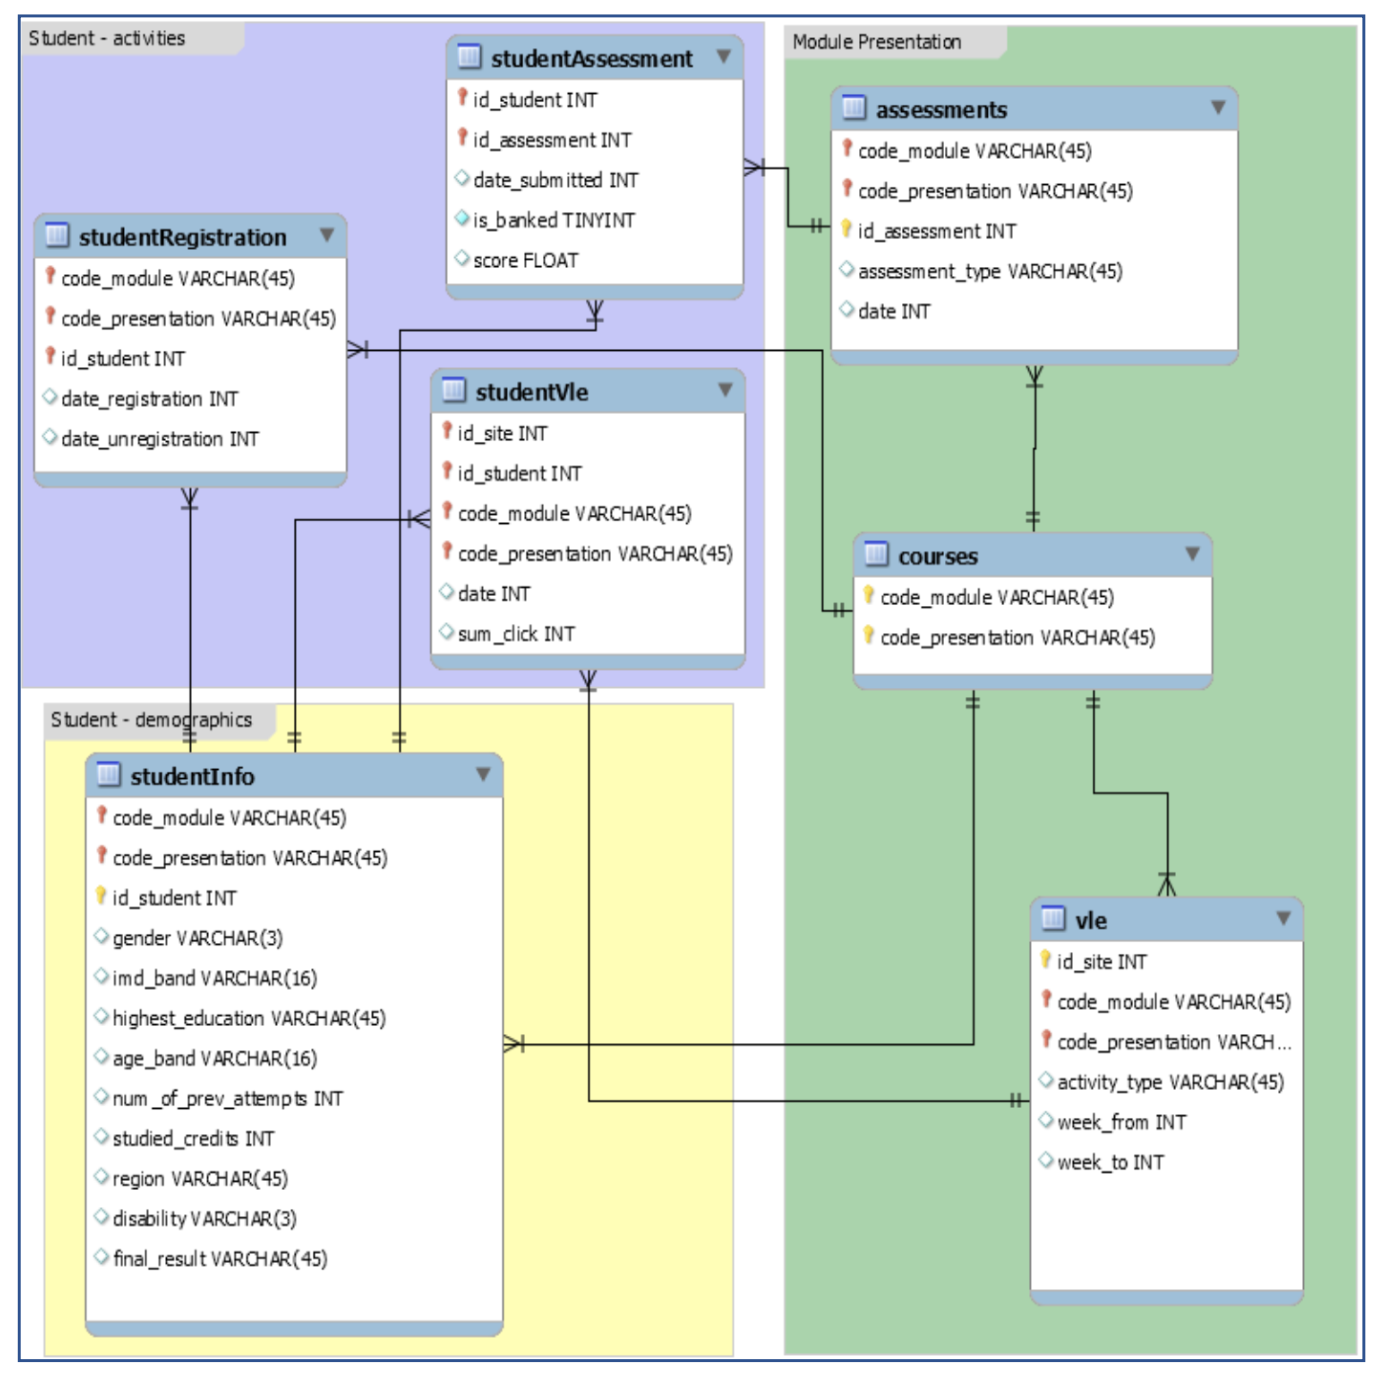
\includegraphics[width=0.9\textwidth]{../Visualizations/Report/2_1_database_scheme.png}
	\caption[Database schema of OULAD dataset]{Database schema of OULAD dataset (reproduced from \cite{nafea_enhancing_2023}).}
	\label{database_scheme}
\end{figure}

\section{Student Engagement Indicators}
Simple, interpretable flags were engineered to capture early excellence and activity in ways that align with common early‑warning practices in learning analytics \cite{macfadyen_mining_2010}.
Mathematical notations are added no understand following equations.

\begin{itemize}
	\item Let $\mathbf{1}[\cdot]$ be the indicator function (1 if the condition is true, else 0).
	\item Let the first graded assessment in a presentation be indexed by $a_1$
	\item Let score $a_1$ be the student’s first‑assessment score (0–100).
	\item Let $date(a_1)$ be its cut‑off day.
	\item Let $C_{pre}$ be the student’s total $sum\_click$ with {\em studentVle.date} $< date(a_1)$.
	\item Let $\mu_{pre}$ be the mean of $C_{pre}$ within the same ($code\_module$, $code\_presentation$).
	\item These columns and date conventions are defined in OULAD.
\end{itemize}

\subsection{Excellent Score Indicator}
A binary indicator for early academic excellence was defined as:
\begin{equation}
	\text{excellent\_Score} = \mathbf{1}\!\left[ \, \text{score}(a_1) \geq 70 \, \right]
	\tag{2.1}
\end{equation}
According to Scholaro database, The Open University awards a “Merit” scale when is higher than $70\%$ \cite{open_university_grading}. This threshold marks, where is categorised as distinction mark for OU, clearly high performance while keeping the rule easy to interpret; early assessment performance has been shown to be informative for final outcomes and targeted support.

\subsection{Active in VLE Indicator}
A binary indicator for above‑average pre‑assessment activity was defined as:
\begin{equation}
	\text{active\_in\_VLE} = \mathbf{1}\!\left[ \, C_{\text{pre}} > \mu_{\text{pre}} \, \right]
	\tag{2.2}
\end{equation}
Clicks prior to the first assessment are counted and compared with the cohort’s mean for the same module‑presentation; VLE click behaviours have repeatedly shown predictive value for course performance, including in OULAD‑based studies \cite{liu_predicting_2023}.

\subsection{Student Engagement Indicator}
A composite engagement flag was defined with a logical OR:
\begin{equation}
	\text{student\_engagement} = \mathbf{1}\!\left[ \, \text{excellent\_Score} = 1 \, \lor \, \text{active\_in\_VLE} = 1 \, \right]
	\tag{2.3}
\end{equation}
This rule fires if either early excellence or above‑average activity is observed, a common, conservative design for early‑warning heuristics that favours recall of potentially successful or engaged students \cite{macfadyen_mining_2010}.

\paragraph{Why these signals}
The pair (grade-based, behaviour-based) captures complementary facets of engagement and aligns with evidence that clickstream engagement and formative performance jointly inform later achievement \cite{baker_benefits_2020}.

\section{Stratification and Encoding}
\subsection{Cohort‑Outcome Stratification}
A stratified hold‑out split was performed per cohort so each module–presentation kept its original class mix, and the target values ({\em Withdrawn/Fail/Pass}) was included in the strata to preserve outcome prevalence within every cohort. Class‑imbalance concerns motivated stratification to reduce variance and avoid misleading metrics on under‑represented outcomes \cite{he_learning_2009}. The split was executed before any encoding to prevent information leakage from validation/test data back into training data \cite{kaufman_leakage_2012}. The implementation relied on scikit‑learn splitters with a fixed random state for reproducibility \cite{pedregosa_scikit-learn_2011}. In the project, three alternatives were examined and Strategy 2 (cohort + outcome) was retained due to its better distribution in comparison with the Strategy 1 (cohort); a triple‑key variant Strategy 3 which include “courses per term” was discarded due to tiny cells that break stratified sampling.

\subsection{Feature Encoding}
Encoding was intentionally minimal and applied only to a selected set of categorical variables that were found relevant for the SDP: $region$, $highest\_education$, $imd\_band$, $age\_band$, and $disability$; numerical and binary features were left unchanged to keep the signal simple. Nominal fields were one‑hot encoded to avoid imposing order, while ordered bands ($imd\_band$, $age\_band$) were ordinal‑encoded to preserve ranks in a compact form \cite{scikit_encoding}. Encoders were fit only on the training split and then applied to the test dataset, with unseen categories mapped safely to an “Unknown” bucket to avoid runtime errors and leakage \cite{scikit_encoding}. The steps were orchestrated with $scikit‑learn$ library and the encoded matrices for the train and test dataset, and labels were persisted for downstream modelling.


\section{Multi-Class Classification}
In education, multi-class classification is complicated since the standard binary techniques are not effective in modelling the interactions among various performance levels, which leads to specialized algorithms \cite{fernandez_learning_2018}. Model collection is in turn influencing the ordinal nature of effects (e.g., from {\em Pass} to {\em Fail}) might need attentive attention at some stage in model training \cite{liu_exploratory_2009}. Standard decomposition methods may bias such type of ordered data, which validate why it is useful to apply native multi-class algorithms in order to predict student performances accurately \cite{krawczyk_learning_2016}.

Class imbalance is a critical challenge in educational data, as traditional accuracy metrics can be misleading by failing to reflect poor performance on key minority classes, such as {\em Withdrawn} students \cite{haixiang_learning_2017}. Proper evaluation of these models requires specialized metrics, such as class-specific recall and macro-averaged F1 scores, to ensure a balanced assessment \cite{luque_impact_2019}. Advanced techniques, including strategic oversampling combined with ensemble methods, have been shown to significantly improve the identification of these at-risk students \cite{galar_review_2012}.

\section{Multi-Class Evaluation Metrics}
The class-specific performance metrics can offer valuable insights on how a model performs and work well for imbalanced data. Among these, precision and recall are core indicators for assessment of classification effectiveness. For a given class $i$, precision is defined as the ratio of true positive predictions to all positive predictions, as shown in Equation 2.1. This concept is introduced in \cite{sokolova_classification_tasks_2009}.
\begin{equation}
	\text{Precision}_{i} = \frac{TP_{i}}{TP_{i} + FP_{i}}
	\tag{2.4}
\end{equation}
\begin{center}
	where $TP_{i}$ represents true positives and $FP_{i}$ represents false positives for class $i$.
\end{center}

On the other hand, recall is defined as the ratio of the actual positive instances that are classified as positive which is given in Equation 2.2 \cite{sokolova_classification_tasks_2009}. In educational applications, recall for the {\em Withdrawn} class is especially important as it measures the model's capacity to detect students who need early support, while having high recall rates ensures that such at-risk students are not missed out even with elevated false positive rates \cite{grandini_metrics_2020}.
\begin{equation}
	\text{Recall}_{i} = \frac{TP_{i}}{TP_{i} + FN_{i}}
	\tag{2.5}
\end{equation}
\begin{center}
	where $TP_{i}$ represents true positives and $FN_{i}$ denotes false negatives for class $i$.
\end{center}

Weighted metrics compensate for the class imbalance by incorporating the relative frequency of each class contributing to the overall performance measure and deliver a model effectiveness evaluation that is more representative of how well it generalizes to all categories \cite{jeni_facing_2013}. Weighted recall is calculated according to the Equation 2.3 \cite{tantisripreecha_novel_2022}.
\begin{equation}
	\text{Weighted Recall} = \sum_{i} w_{i} \times \text{Recall}_{i}
	\tag{2.6}
\end{equation}
\begin{center}
	where $w_{i}$ is the weight for class $i$, usually based on its frequency in the dataset.
\end{center}

Weighted F1-score is the harmonic mean of precision and recall for each class $i$ \cite{tantisripreecha_novel_2022} \cite{opitz_closer_2024} as in the Equation 2.4. These balanced metrics allow us to measure the performance level for all categories of evaluation indicators while still being sensitive to the practical important of minority class detection in the educational intervention systems \cite{krawczyk_learning_2016}.
\begin{equation}
	\text{Weighted F1} = \sum_{i} w_{i} \times F1_{i}
	\tag{2.7}
\end{equation}
\begin{center}
	where $F1_{i} = 2 \times \frac{\text{Precision}_{i} \times \text{Recall}_{i}}{\text{Precision}_{i} + \text{Recall}_{i}}$ 
	and $w_{i}$ represents the weight assigned to class $i$.
\end{center}

\section{Strategies for Imbalanced Data}
\label{sec:strategies_imbalanced_data}
Balanced class weight is one of the basic approaches to address the imbalance of the dataset where the importance of each class is adjusted automatically and inversely proportional to the frequency of that class and the mathematical foundation is given as it is written in the Equation 2.5 \cite{akor_hierarchical_2025}.
\begin{equation}
	w_{i} = \frac{n_{\text{samples}}}{n_{\text{classes}} \times n_{\text{samples}_{i}}}
	\tag{2.8}
\end{equation}
\begin{center}
	where $w_{i}$ denotes the weight for class $i$, $n_{\text{samples}}$ represents the total number of samples, 
	$n_{\text{classes}}$ indicates the number of classes, and $n_{\text{samples}_{i}}$ represents the number of samples in class $i$.
\end{center}

Customized scoring metrics deepen this approach by considering domain-specific preferences, by dropout-specific optimization forcing the maximization of the recall for withdrawal detection via biasing the learning criterion in favour of at-risk students and focusing less on false negatives \cite{orooji_predicting_2019}.

Early warning signs do exist to prevent high-risk youngsters and to intervene early. In the context of dropout prediction, the imbalance class is the minority dropout class, which results in heavy emphasize on recall to detect the dropout students for timely intervention \cite{lee_machine_2019}. Unbalanced-learning techniques (e.g., resampling or class weighting) generally improve recall for the rare class (dropout) at the expense of precision \cite{orooji_predicting_2019}, which is the same precision-recall trade-off this work aims to find the best level of.

In the area of dropout early-detection, balancing the class distribution among minority and majority instances should be considered desirably by using class weights, which disadvantage the majority and advantage the minority class, e.g., the weight of the minority class being higher than $1$ and the weight of the majority class being equal to $1$ is common \cite{hlosta_ouroboros_2017}. More recent losses, e.g., the Class-Balanced Loss, have tried to provide a more principled re-weighting beyond naïve inverses only when classes are long-tailed \cite{cui_class-balanced_2019}. For the current study it is beneficial as we would like to investigate alternative to ad-hoc multipliers, used for balanced weighting, like x$1.2$ for the minority class {\em Withdrawn} and x$0.8$ for the majority class {\em Pass}. The multipliers are domain specific choices of the experimentations: there is one setting that uses no multipliers (balanced weighting), and one that applies the multipliers. Lastly, note that overall accuracy may be deceptive of imbalanced data, as Precision and Recall can better assess minority-class detection quality \cite{saito_precision-recall_2015}.

\section{ML Algorithms for SDP}
Ensemble learning exploits multiple models to reduce variance and improve generalization; in RF, bootstrap aggregation (bagging) draws resamples of the training set and averages randomized decision trees, providing robustness and out‑of‑bag error estimation \cite{breiman_bagging_1996} \cite{breiman_rf_2001}. Feature importance in RF is commonly derived from impurity decreases or permutation‑based accuracy drops, enabling screening of influential predictors in heterogeneous educational data \cite{breiman_rf_2001}. Gradient‑boosting frameworks fit weak learners sequentially under an additive model to minimize a differentiable loss, while LightGBM accelerates this process using histogram‑based splits, leaf‑wise growth, and gradient‑based one‑side sampling for scalability on high‑dimensional, large cohorts \cite{friedman_gbm_2001} \cite{ke_lightgbm_2017}. LR models the log‑odds of class membership and estimates coefficients by maximum likelihood, yielding interpretable effects as odds ratios and supporting regularization for stability when features are correlated \cite{cox_regression_1958} \cite{nelder_generalized_1972}. SVM maximise the geometric margin via convex quadratic programming and use kernel mappings to induce flexible non‑linear decision boundaries while controlling capacity through the margin and kernel parameters \cite{cortes_svm_1995}. 

Instance‑based learning with KNN classifies by a majority (plurality) vote among the K closest samples, so decision boundaries are local and sensitive to the choice of distance metric and K, with common metrics including Euclidean, Manhattan, and Mahalanobis distances \cite{cover_nearest_1967} \cite{aha_instance-based_1991}. Multi‑layer perceptrons (a type of NN) compose affine transformations with non‑linear activations and are trained end‑to‑end by backpropagation to minimize a supervised loss, with universal approximation guaranteeing expressive capacity under sufficient width or depth \cite{rumelhart_learning_1986} \cite{hornik_multilayer_1989}. These foundations motivate comparing RF, LightGBM, LR, SVM, KNN, and NN for dropout prediction, balancing interpretability, non‑linear modelling power, and computational efficiency under class imbalance typical of at‑risk cohorts \cite{krawczyk_learning_2016}.

\section{Model Evaluation and Comparison Methodologies}
Performance was estimated with stratified 5‑fold cross‑validation \cite{kohavi_study_1995} on the training split to preserve class proportions and reduce variance in imbalanced data, with a fixed stratified train–test split reused for all models to ensure comparability \cite{luque_impact_2019}. Hyperparameter search was executed within cross‑validation (GridSearchCV) and final metrics were computed once on the untouched test split to limit selection bias \cite{varma_bias_2006}. All models were evaluated on identical folds and scoring rules to enable fair, paired comparisons across the pipeline \cite{demsar_statistical_2006}. Hyperparameters were optimized via exhaustive GridSearchCV with five folds, parallel execution, dropout‑recall as the objective, and class‑weighting to emphasize minority cases \cite{kohavi_study_1995} \cite{krawczyk_learning_2016}.

Regularisation and early stopping are treated as crucial mechanisms to curb over‑fitting and stabilise learning dynamics \cite{prechelt_early_2012}. In LR, the strength of regularisation is controlled by the inverse‑penalty parameter $C$, with $L1/L2$ penalties shaping sparsity and shrinkage behaviour \cite{ng_feature_2004}. For SVM, the soft‑margin constant $C$ and kernel scale gamma are tuned to balance margin violations and function smoothness \cite{cortes_svm_1995}. In decision trees and ensemble methods, maximum depth and the number of estimators are adjusted to limit variance and improve robustness \cite{breiman_rf_2001}. In gradient boosting, the learning rate and number of boosting rounds jointly govern additive model capacity and error reduction \cite{friedman_gbm_2001}. For KNN, the neighbourhood size $k$ and the choice of distance metric determine locality and boundary smoothness \cite{cover_nearest_1967}. In multilayer perceptrons, hidden‑layer size and weight decay are set under backpropagation to control capacity and enhance generalisation \cite{krogh_simple_1991}. 

% -----------------------------------------------------------------------------

\chapter{Methodology and Implementation}
\label{chap:execution}

\vspace{1cm} 
\noindent
This chapter describes the methodical process used to create and assess ML models for student dropout prediction, covering everything from data preprocessing to model deployment and validation.

\section{Overview and Research Design}
With an emphasis on early intervention capabilities, this study applies a ML pipeline intended to forecast the likelihood of student dropout in online learning environments. By creating predictive models that can identify at-risk students before they drop out of their courses, the study tackles the crucial problem of student retention in higher education.

\section{Data Class Distribution}
The class distribution of the cleaned and merged dataset, which comprises three outcome categories, is shown in Table~\ref{tab:class_distribution_merge}. There are $27,725$ records in all in the dataset. There is a glaring class imbalance in the distribution: the frequency of {\em Fail} outcomes is closer to {\em Withdrawn} than to {\em Pass}, while the number of {\em Withdrawn} outcomes is much lower than that of {\em Pass} outcomes.
\begin{table}[h!]
	\centering
	\begin{tabular}{|l|r|r|r|}
		\hline
		\textbf{} & \textbf{Withdrawn (Class 0)} & \textbf{Fail (Class 1)} & \textbf{Pass (Class 2)} \\
		\hline
		Counts       & 5,296 & 7,044 & 15,385 \\
		\hline
		Percentages  & 19.1\% & 25.4\% & 55.5\% \\
		\hline
	\end{tabular}
	\caption{Data Class Distribution}
	\label{tab:class_distribution_merge}
\end{table}


\subsection{Research Methodology Framework}
The approach uses supervised learning and compares six different ML in a methodical manner: RF, Multinomial LR, KNN, LightGBM Gradient Boosting, SVM, and NN. Robust evaluation across various learning paradigms, ranging from distance-based and deep learning approaches to ensemble methods and linear models, is ensured by this thorough algorithmic comparison.

From data intake to model winning selection, the research framework uses a structured pipeline (Figure~\ref{project_pipeline}), integrating modular Python architecture for scalability and reproducibility. Each algorithm undergoes rigorous hyperparameter optimisation using GridSearchCV with 5-fold cross-validation to guarantee fair comparison and optimal performance extraction.

\subsection{Dropout Optimization}
To enable successful early intervention systems, the main goal is to maximise dropout recall to $\geq60\%$. Since false negatives, or missing {\em Withdrawn} students, have more serious repercussions than false positives, or failing students who might succeed, in educational intervention contexts, this metric gives priority to identifying students who will drop out. In order to balance practical resource constraints with effective early intervention capabilities, the $60\%$ threshold was set especially for this project. This ensures that roughly two-thirds of {\em Withdrawn} students are identified while maintaining manageable caseloads for institutional support services.

\subsection{Class Imbalance Challenge}
With $19.1\%$ dropout students (minority class), $25.4\%$ failing students, and $55.5\%$ passing students (majority class), the dataset represents a serious class imbalance issue. Specific optimisation techniques, such as unique class weighting schemes and dropout-focused evaluation metrics, are needed to address this imbalance. By using class weights of roughly $2.09$x for dropouts, $1.31$x for failures, and $0.48$x for passes across various algorithms, the research employs customised strategies to make sure minority class detection is not overpowered by majority class dominance.

\begin{figure}[t]
	\centering
	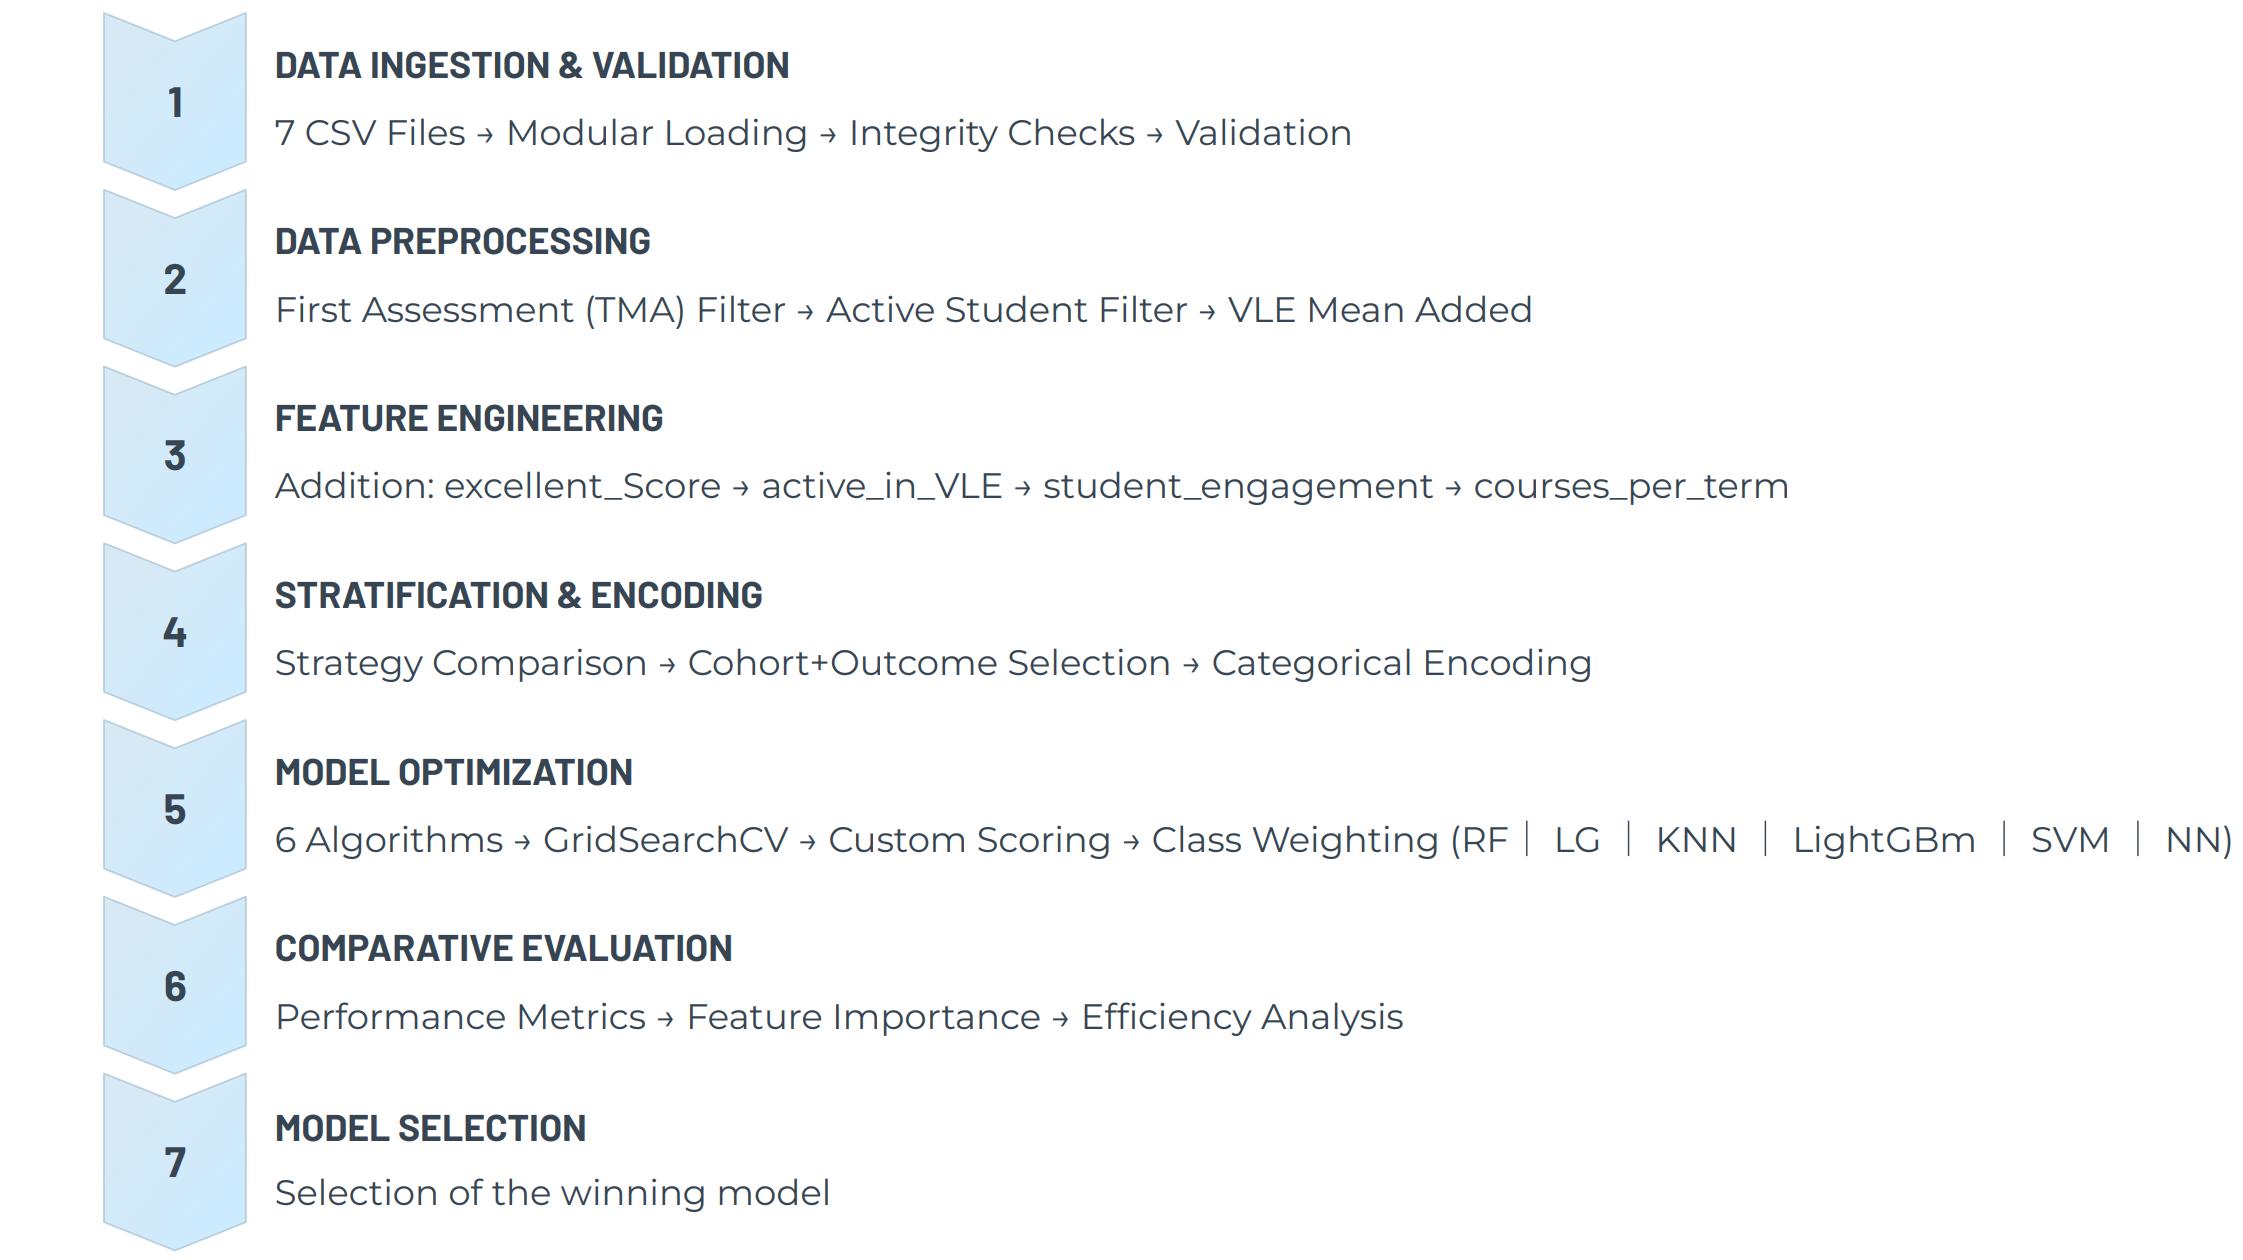
\includegraphics[width=0.9\textwidth]{../Visualizations/Report/3_1_project_pipeline.png}
	\caption{The Seven-Phase Project Pipeline}
	\label{project_pipeline}
\end{figure}

\section{Data Architecture and Modular Design}
As shown in Figure~\ref{project_pipeline}, the implementation uses a methodical seven-phase pipeline architecture intended for comprehensive SDP. From the intake of raw data to the deployment of models, this modular design guarantees repeatable processes while preserving data integrity across the ML pipeline.

\subsection{Phase 1: Data Ingestion and Validation}
Seven CSV files containing learning analytics data are automatically loaded at the start of the pipeline. Validation protocols check column structures and data integrity.

\subsection{Phase 2: Data Preprocessing}
Predictive modelling is based on core data transformations. By determining the earliest {\em TMA} (Tutor Marked Assessment) dates for each course-presentation combination, assessment filtering establishes standardised prediction windows for early intervention. Consistency across diverse data sources is ensured by data type conversions and missing value handling. Only participants who are actively participating during assessment periods are kept by student filtering protocols, which eliminate inactive participants.

\subsection{Phase 3: Feature Engineering}
From raw learning analytics, sophisticated feature creation algorithms produce predictive indicators. Before assessment deadlines, click-stream data is compiled by VLE engagement metrics to identify patterns in behaviour. Academic performance indicators establish engagement thresholds and binary flags for excellence (scores $\geq70$). The $courses\_per\_term$ feature provides context for student capacity analysis by quantifying the distribution of academic load.

\subsection{Phase 4: Stratification and Encoding}
Advanced stratification techniques preserve demographic representation while maintaining class proportions across cohort boundaries. With $19.1\%$ dropout representation, the chosen cohort+outcome strategy guarantees balanced train-test splits. The specific transformations used in categorical encoding are binary encoding for dichotomous variables, ordinal encoding for hierarchical relationships, and one-hot encoding for nominal variables.

\subsection{Phase 5: Model Optimization}
Using thorough hyperparameter optimisation, a systematic algorithm comparison assesses six different ML techniques. 5-fold cross-validation in GridSearchCV guarantees equitable comparison across various learning paradigms. Custom scoring metrics use specific weighting strategies to manage class imbalance while giving priority to dropout recall optimisation.

\subsection{Phase 6: Comparative Evaluation}
A thorough model evaluation analyses performance across six algorithms using a variety of visualisation techniques. Direct performance comparison is made possible by horizontal bar charts that compare key metrics (dropout recall, dropout precision, at-risk recall, weighted F1). Multi-metric performance profiles for each model are displayed using five-dimensional radar plots, which also highlight the models' advantages and disadvantages. Runtime efficiency scatter plots determine the best algorithms for various deployment scenarios by analysing trade-offs between computational cost and performance. With comprehensive confusion matrices for every algorithm, three-panel performance dashboards categorise models into three performance tiers: Excellent $\geq60\%$, Good $40-60\%$, and Needs Work $<40\%$.

\subsection{Phase 7: Model Selection}
The comparative analysis in Phase 6 is the source of the systematic evaluation criteria used in evidence-based model selection. Dropout recall performance ($\geq60\%$ threshold), computational efficiency, and deployment feasibility are given top priority during the selection process. With a $66.84\%$ dropout recall, superior efficiency (4-minute training time), and interpretability advantages, LR is the best option. Runtime efficiency analysis, practical deployment considerations, and performance tier classification (Excellent, Good, Needs Work) are among the selection criteria. While underperforming algorithms (NN at $18.67\%$ recall) are not taken into consideration for production, runner-up models (SVM with $63.09\%$ recall) offer backup options. The final choice strikes a balance between operational needs for actual educational intervention systems and predictive performance.

\section{Data Preprocessing and Feature Engineering}
A systematic six-stage pipeline is implemented by the data preprocessing and feature engineering phases (Phase $2$ and Phase $3$ in Figure~\ref{project_pipeline}), which convert raw learning analytics into predictive features for early intervention systems (Figure~\ref{features_pipeline}). Prior to determining academic outcomes, this creates behavioural indicators and temporal prediction windows that capture patterns of student engagement.

\subsection{Stage 1: Integrating Data Sources}
The pipeline starts with the thorough integration of five main data sources: student registrations, VLE interaction logs, assessment structure and student assessment metadata, and demographic data. The original dataset includes over $10$ million VLE interactions and $32,593$ student registrations across $22$ courses.

\subsection{Stage 2: Defining the Initial Assessment Period}
\label{subsec:defining_TMA}
For every course-presentation combination, this stage identifies the first {\em TMA} dates. In order to determine the earliest assessment dates for $22$ courses, this processes $106$ {\em TMA} assessments. By eliminating participants who withdrew prior to their initial assessment opportunity, active student filtering guarantees that attention is directed towards students who might profit from intervention. Consequently, $27,725$ students in total match these filters.

\subsection{Stage 3: Extracting Behavioural Features}
Up until the initial evaluation, this stage shows how three fundamental behavioural dimensions (VLE interaction, academic performance, and course load), were extracted. In order to determine the total and average clicks per student in relation to a course-presentation baseline, VLE interaction analysis analyses $2,587,468$ clicks that took place prior to the first assessment deadlines. Academic performance extraction uses a merit threshold analysis (threshold $70$) and records the initial assessment results. Students taking multiple concurrent courses are identified through course load quantification, which also provides context for their academic capacity. For this data, the maximum number of concurrent courses is $2$; it was not found students with three or more courses at the same presentation time.

\subsection{Stage 4: Creating Indicator}
The fourth step filters the $27,725$ students and converts continuous behavioural measures into interpretable binary indicators. Merit-level performance ($\geq70$ points) is attained by $16,687$ students ($60.2\%$ of the total) according to the academic excellence classification ($excellent\_Score$). $9,870$ students ($35.6\%$) whose platform engagement surpasses course-specific averages are flagged by the VLE activity classification ({\em active\_in\_VLE}). Additionally, a course load analysis ($courses\_per\_term$) was added to quantify the academic workload of $1,270$ students ($4.6\%$) who are managing multiple concurrent courses.

\subsection{Stage 5: Aggregating an Engagement Indicator}
In stage five, various pathways to academic success are captured by combining individual indicators into composite measures. By using logical OR operations to combine academic excellence and VLE activity, the unified engagement feature ($student\_engagement$) finds $19,932$ students ($71.9\%$) who are either performing well or showing strong platform engagement. This composite approach acknowledges that various engagement patterns may lead to students' success.

\subsection{Stage 6: Engineering the Final Training Dataset}
The last step of data preparation creates a validated, ML-ready dataset of $27,725 students$ and $25$ features by combining preprocessed data with engineered behavioural and demographic features. The distribution of classes in this dataset is $55.5\%$ {\em Pass}, $25.4\%$ {\em Fail}, and $19.1\%$ {\em Withdrawn}. With the {\em Withdrawn} students representing a crucial minority class, it draws attention to the problem of class imbalance. Now that the dataset has been cleaned and optimised, it is ready for the next round of ML pipelines, where specific techniques will be used to predict outcomes for this important minority group.

\begin{figure}[h]
	\centering
	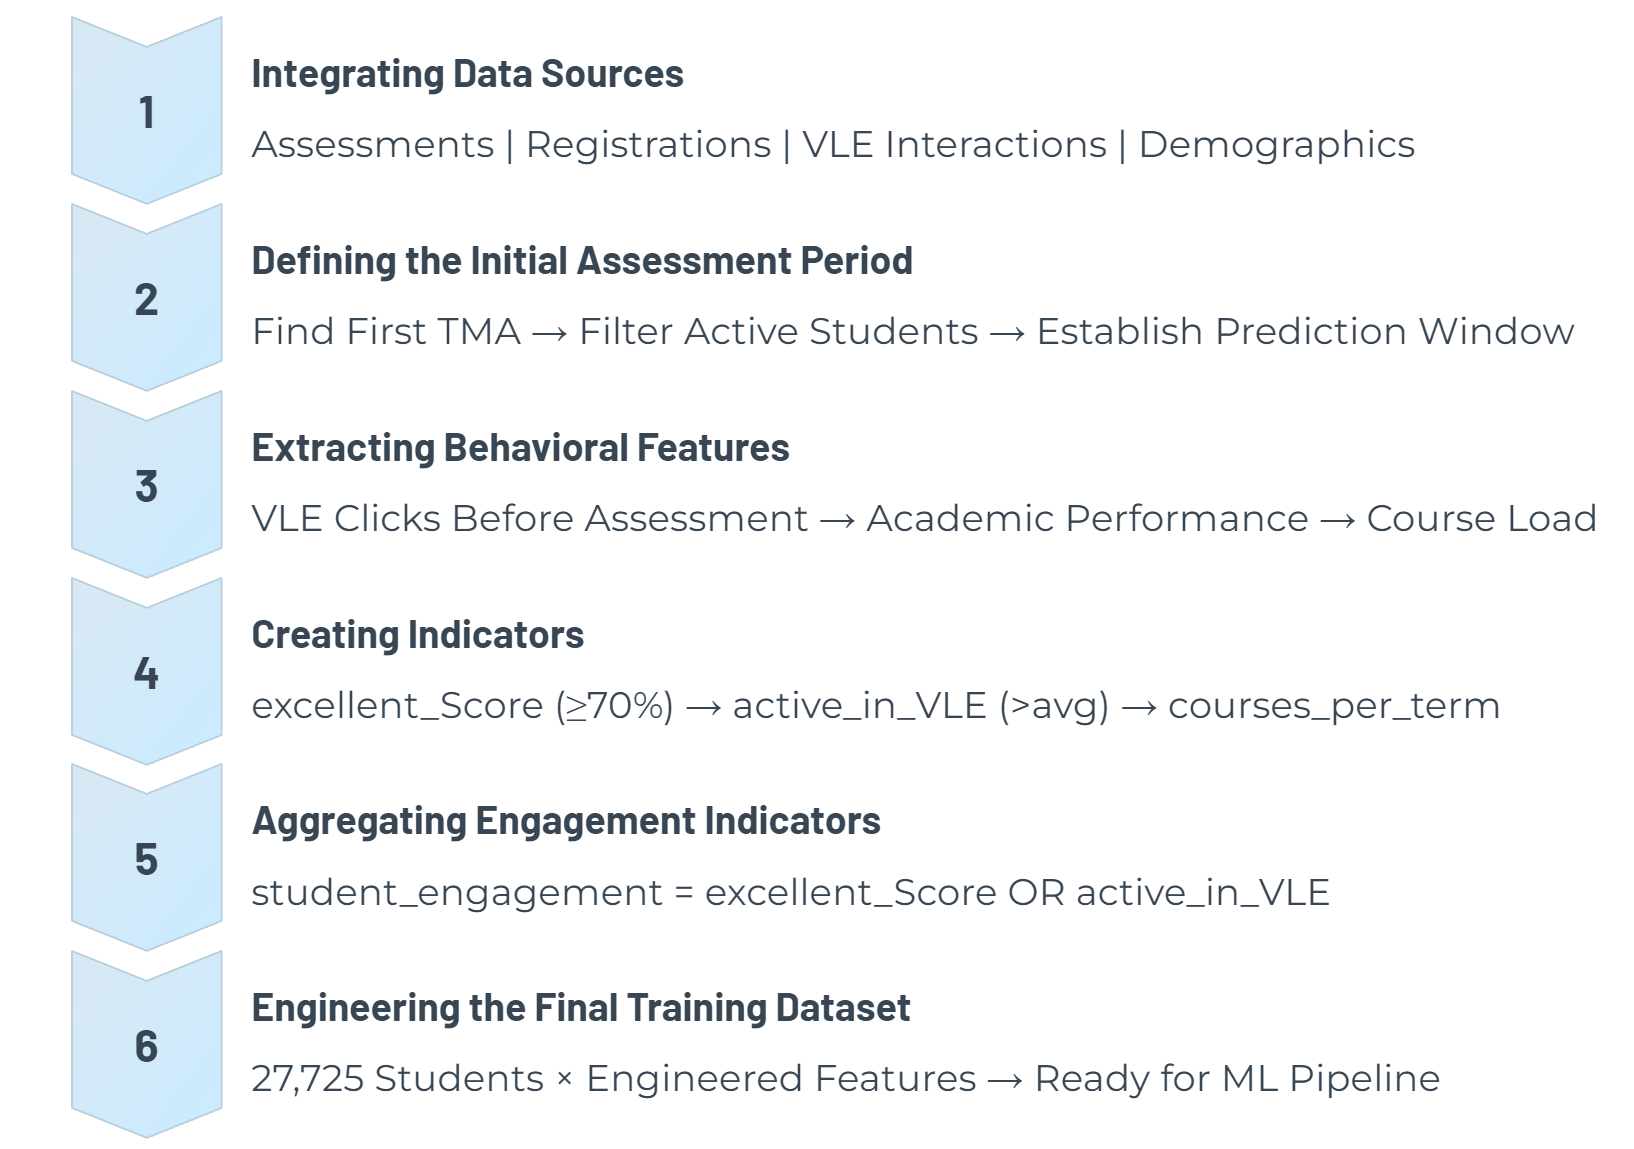
\includegraphics[width=0.9\textwidth]{../Visualizations/Report/3_2_features_pipeline.png}
	\caption{The Six-Stage Engineering Feature Pipeline}
	\label{features_pipeline}
\end{figure}

\section{Data Stratification Strategy}
\label{sec:data_stratification}
Three stratification techniques are evaluated methodically to maximise the preservation of class distribution. Using course-presentation combinations, Strategy 1 uses basic cohort-based stratification. Using a combination of cohort and outcome stratification, Strategy 2 maintains the distributions of academic outcomes and demographics. Triple stratification using cohort$+$outcome$+$courseload variables is attempted in Strategy 3.

\paragraph{Strategy Selection:} Comparative analysis shows that Strategy 2 (Cohort + Outcome) is the best course of action. Since many cohort-outcome-courseload combinations contain only one student, triple stratification (Strategy 3) fails because combined groupings have insufficient sample sizes. As shown in Table~\ref{tab:class_distribution}, Strategy 2 effectively preserves the crucial $19.1\%$ dropout representation across train-test splits while maintaining class proportions.

\paragraph{Stratified Sampling Implementation:}  The chosen strategy guarantees equitable representation for both academic results and course cohorts. The train-test split allocation maintains proportional class representation by using a $80\%-20\%$ distribution. This approach ensures sufficient samples for minority class optimisation in later model training stages while maintaining demographic diversity.

\begin{table}[h]
	\centering
	\begin{tabular}{|l|c|c|c|c|}
		\hline
		\textbf{Strategy} & \makecell{\textbf{Withdrawn} \\ \textbf{(Class 0)}} & \makecell{\textbf{Fail} \\ \textbf{(Class 1)}} & \makecell{\textbf{Pass} \\ \textbf{(Class 2)}} & \textbf{Status} \\
		\hline
		Original Dataset & 19.1\% & 25.4\% & 55.5\% & Baseline \\
		\hline
		Strategy 1: Cohort Only & 19.3\% & 25.0\% & 55.7\% & Acceptable \\
		\hline
		Strategy 2: Cohort + Outcome & 19.1\% & 25.4\% & 55.5\% & \textbf{Selected} \\
		\hline
		Strategy 3: Cohort + Outcome + Courseload & - & - & - & Failed \\
		\hline
	\end{tabular}
	\caption{Class Distribution Comparison Across Stratification Strategies}
	\label{tab:class_distribution}
\end{table}

\section{Feature Selection for ML Models}
In order to find variables with significant predictive relationships for predicting student outcomes, the feature selection process used exploratory data analysis. It also methodically looked at socio-demographic traits and engineered features to maximise model performance while preserving interpretability. Table~\ref{tab:sociodemographic} provides more information on these variables.

\begin{table}[h!]
	\centering	
	\begin{tabular}{|l|l|p{8cm}|}
		\hline
		\textbf{Variable} & \textbf{Type} & \textbf{Categories} \\ \hline
		\textbf{Gender} & Binary & Female, Male \\ \hline
		\textbf{Age Band} & Ordinal & 0--35, 35--55, 55+ \\ \hline
		\textbf{Disability} & Binary & No, Yes \\ \hline
		\textbf{Highest Education} & Ordinal & No Formal $\rightarrow$ Post Graduate (5 levels) \\ \hline
		\textbf{IMD Band} & Ordinal & 10 income deprivation percentiles \\ \hline
		\textbf{Region} & Nominal & 13 UK geographical regions \\ \hline
	\end{tabular}
	\caption{Socio-Demographic Variable Characteristics}
	\label{tab:sociodemographic}
\end{table}

Six socio-demographic factors were subjected to linear regression analysis in order to measure their associations with student outcomes. Proportional distributions among the three outcome classes ({\em Pass, Fail, and Withdrawn}) were examined, and $R^2$ coefficients and slope measurements were used to evaluate the relevance of the variables. Table~\ref{tab:var_selection} displays a summary of the regression's results with $R^2$ and the corresponding slope for each class and variable selection.

Additional visual information about this regression can be found in Appendix~\ref{appx:socio_demographic_plots}, which displays six plots for these socio-demographic variables. A summary of the findings from those plots is included here. The analysis showed that gender had perfect mathematical relationships ($R^2$ $1.000$) but minimal practical differences between female and male students ($18.0\%$ vs $20.0\%$ withdrawal rates, $57.1\%$ vs $54.1\%$ pass rates), which led to its exclusion from model training. Strong correlations were found between Age Band ($R^2$ $0.993-1.000$), with older students exhibiting increasingly better results. Pass rates rose sharply from $53.5\%$ to $68.2\%$, while withdrawal rates dropped from $19.5\%$ ($0-35$ years) to $16.9\%$ ($55+$ years). With pass rates rising from $38.7\%$ to $70.9\%$ and withdrawal rates falling from $25.6\%$ (no qualifications) to $17.3\%$ (post-graduate), the strongest substantive predictor ($R^2$ $0.788-0.984$) was highest education. Strong socioeconomic relationships were found by IMD Band ($R^2$ $0.819-0.948$), with pass rates rising from $43.6\%$ to $65.0\%$ as deprivation decreased and withdrawal rates for students from the most deprived areas being $22.0\%$ compared to $16.3\%$ in the least deprived areas. Disability Status demonstrated perfect mathematical relationships ($R^2$ $1.000$) with significant practical implications; students with disabilities had lower pass rates ($45.8\%$ vs. $56.5\%$) and much higher withdrawal rates ($27.3\%$ vs. $18.2\%$). Although region showed little variation and weak relationships ($R^2$ $0.010-0.040$), it was kept to account for regional differences in educational access that were not represented by other variables.

\begin{table}[h!]
	\centering
	\begin{tabular}{|l|cc|cc|cc|l|}
		\hline
		\multirow{3}{*}{\textbf{Variable}} & \multicolumn{6}{c|}{\textbf{Class}} & \multirow{3}{*}{\shortstack{\textbf{Selection}\\\textbf{Decision}}} \\
		\cline{2-7}
		& \multicolumn{2}{c|}{\textbf{Withdrawn}} & \multicolumn{2}{c|}{\textbf{Fail}} & \multicolumn{2}{c|}{\textbf{Pass}} & \\
		\cline{2-7}
		& \textbf{R$^2$} & \textbf{Slope} & \textbf{R$^2$} & \textbf{Slope} & \textbf{R$^2$} & \textbf{Slope} & \\
		\hline
		\textbf{Gender}            & 1.000 & +0.020 & 1.000 & +0.011 & 1.000 & -0.030 & \textbf{Excluded} \\
		\textbf{Age Band}          & 1.000 & -0.013 & 0.994 & -0.061 & 0.996 & +0.074 & \textbf{Included} \\
		\textbf{Disability}        & 1.000 & +0.091 & 1.000 & +0.018 & 1.000 & -0.107 & \textbf{Included} \\
		\textbf{Highest Education} & 0.788 & -0.021 & 0.984 & -0.060 & 0.966 & +0.081 & \textbf{Included} \\
		\textbf{IMD Band}          & 0.819 & -0.001 & 0.909 & -0.002 & 0.948 & +0.002 & \textbf{Included} \\
		\textbf{Region}            & 0.010 & +0.000 & 0.036 & +0.002 & 0.040 & -0.002 & \textbf{Included} \\
		\hline
	\end{tabular}
	\caption{Model fit $R^2$ and slope by variable across outcome classes.}
	\label{tab:var_selection}
\end{table}

By identifying behavioural and performance patterns not found in raw demographic data, the six-stage feature engineering pipeline (Figure~\ref{features_pipeline}) produced four key variables that complemented socio-demographic characteristics:  $student\_engagement$ (binary composite engagement that meets either excellence or VLE activity criteria), {\em active\_in\_VLE} (binary above-average virtual learning engagement prior to first assessment), $excellent\_Score$ (binary academic merit threshold indicator for $\geq70\%$ performance), and $courses\_per\_term$ (continuous academic load distribution reflecting study intensity patterns).

\section{Categorical Encoding Strategy}
Using the $encoding\_utils$ module, tailored encoding techniques handle various categorical variable types. Region variables are treated as nominal categories with no intrinsic ordering through one-hot encoding. Ordinal encoding is used to preserve hierarchical relationships across socioeconomic and demographic dimensions while maintaining ranked sequences for the variables of education, age, and IMD band. For dichotomous classification, disability status uses binary encoding. Maintaining feature alignment and preventing data leakage are achieved by encoding consistency across train-test splits. Table~\ref{tab:encoding_strategy} provides an overview of this.

\paragraph{Dataset Export} Systematic model comparison is made possible by encoded datasets exporting as standardised CSV files ($X\_train\_encoded.csv$, $X\_test\_encoded.csv$, $y\_train.csv$, $y\_test.csv$). The encoding procedure preserves the temporal validity set in earlier preprocessing stages while generating consistent feature matrices appropriate for a range of algorithm requirements.

\begin{table}[h]
	\centering
	\begin{tabular}{|c|c|c|}
		\hline
		\textbf{Variable Type} & \textbf{Variables} & \textbf{Encoding Method} \\
		\hline
		Nominal & Region & One-Hot Encoding \\
		\hline
		Ordinal & Education, Age, IMD Band & Ordinal Encoding \\
		\hline
		Binary & Disability & Binary Encoding \\
		\hline
	\end{tabular}
	\caption{Encoding Strategy Matrix}
	\label{tab:encoding_strategy}
\end{table}

\section{Class Weighting Strategy}
\label{sec:class-weighting}
Class imbalance in educational datasets, where {\em Withdrawn} students make up only $19.1\%$ of the dataset population, requires strategic weighting methods that are implemented through a two-stage calculation process that combines custom multipliers with sklearn's balanced weighting. First, balanced weights are calculated using sklearn's $compute\_class\_weight('balanced')$ function to produce baseline values proportional to inverse class frequencies. Next, strategic multiplier application is applied to improve dropout detection capabilities. This is demonstrated in Algorithm~\ref{alg:custom_weights}, where the multiplier values ($1.2$x, $1.0$x, $0.8$x) were chosen to reduce majority class dominance by 20\% and increase dropout class sensitivity by 20\%. These multiplier values were selected especially for this project and can be altered to improve the recall metric or other pertinent metrics, depending on the stakeholders' domain expertise. With this setup, the class balance is changed from the initial balanced weights $\{0: 1.74, 1: 1.31, 2: 0.60\}$ to the optimised custom weights $\{0: 2.09, 1: 1.31, 2: 0.48\}$.

\begin{algorithm}[h]
	\KwIn{$y\_train$, $classes$}
	\KwOut{Custom class weights}
	
	$balanced\_weights \leftarrow compute\_class\_weight(`balanced', classes, y\_train)$\;
	
	$custom\_weights \leftarrow \{ $\;
	\Indp
	$0 : balanced\_weights[0] \times 1.2$ \tcp{Dropout class boost}	
	$1 : balanced\_weights[1] \times 1.0$ \tcp{Fail class unchanged}	
	$2 : balanced\_weights[2] \times 0.8$ \tcp{Pass class reduction}
	\Indm
	$\}$\;
	
	Resulting weights: $\{0: 2.09, 1: 1.31, 2: 0.48\}$\;
	
	\caption{Computation of custom class weights for ML training.}
	\label{alg:custom_weights}
\end{algorithm}

\subsection{Class Weight implementation}
Three different categories based on native support capabilities are revealed by class weight implementation across six chosen algorithms, as shown in Table~\ref{tab:class_weight}. Through built-in $class\_weight$ parameters that automatically modify loss functions and sample importance during training, RF, LG, LightGBM, and SVM offer direct implementation. Because of its distance-based architecture, KNN has limited implementation capabilities and does not support native class weights. Custom weights can be declared, but they are not successfully integrated during prediction. With no alternative strategies like weighted sampling or custom loss functions implemented in the examined notebooks, NN ($MLPClassifier$) is still unsupported and expressly lacks class weight functionality.

\begin{table}[h]
	\centering
	\begin{tabular}{|l|c|l|l|}
		\hline
		\textbf{Algorithm} & \textbf{Native Support} & \textbf{Implementation Method} & \textbf{Usage Status} \\
		\hline
		Random Forest           & $\checkmark$ & \texttt{class\_weight} parameter & \textbf{Active} \\
		\hline
		Logistic Regression     & $\checkmark$ & \texttt{class\_weight} parameter & \textbf{Active} \\
		\hline
		LightGBM                & $\checkmark$ & \texttt{class\_weight} parameter & \textbf{Active} \\
		\hline
		Support Vector Machine  & $\checkmark$ & \texttt{class\_weight} parameter & \textbf{Active} \\
		\hline
		K-Nearest Neighbours     & $\times$     & Use another type of weighting          & \textbf{Not applied} \\
		\hline
		Neural Networks         & $\times$     & Not supported by MLPClassifier   & \textbf{Not applied} \\
		\hline
	\end{tabular}
	\caption{Class Weight Support by ML model}
	\label{tab:class_weight}
\end{table}

\section{Custom Dropout-Focused Scoring Metrics}
The three-class imbalanced nature of student outcome prediction necessitates specialised metrics that emphasise early identification of {\em Withdrawn} students. This led to the development of custom dropout-focused scoring functions to supplement a baseline evaluation framework of seven traditional $sklearn$ metrics that provide balanced perspectives on classification performance across precision, recall, and F1-score dimensions. Standard ML evaluation metrics prioritise overall classification accuracy. Table~\ref{tab:std_metrics} provides an appreciation of these standard metrics.

To separate performance measurement for the minority {\em Withdrawn} class (Class 0) and {\em Fail} student populations in student dropout prediction, three specialised scoring functions were created. Its addition is also visible in the Algorithm~\ref{alg:custom_dropout_scorers}, where the ML model to be used for training is the input estimator.

\begin{table}[h]
	\centering
	\begin{tabular}{|l|l|l|l|}
		\hline
		\textbf{Metric} & \textbf{Function} & \textbf{Scope} & \textbf{Purpose} \\
		\hline
		\texttt{accuracy}            & Overall classification rate & Global      & General performance measure \\
		\hline
		\texttt{f1\_weighted}        & Weighted F1-score           & Multi-class & Class-size adjusted F1      \\
		\hline
		\texttt{f1\_macro}           & Unweighted F1-score         & Multi-class & Equal class importance      \\
		\hline
		\texttt{precision\_weighted} & Weighted precision          & Multi-class & Class-size adjusted precision \\
		\hline
		\texttt{recall\_weighted}    & Weighted recall             & Multi-class & Class-size adjusted recall  \\
		\hline
		\texttt{precision\_macro}    & Unweighted precision        & Multi-class & Equal class precision       \\
		\hline
		\texttt{recall\_macro}       & Unweighted recall           & Multi-class & Equal class recall          \\
		\hline
	\end{tabular}
	\caption{Standard Evaluation Metrics}
	\label{tab:std_metrics}
\end{table}

\begin{algorithm}[h]
	\KwIn{$estimator$, $X$, $y$}
	\KwOut{Custom scoring functions for Withdrawn and Fail students}
	
	\textbf{Function dropout\_recall}($estimator, X, y$): \\
	\Indp
	$y\_pred \leftarrow estimator.predict(X)$\;
	\Return $recall\_score(y, y\_pred, labels=[0], average=`macro')$ \tcp*{class 0 recall}
	\Indm
	
	\textbf{Function dropout\_precision}($estimator, X, y$): \\
	\Indp
	$y\_pred \leftarrow estimator.predict(X)$\;
	\Return $precision\_score(y, y\_pred, labels=[0], average=`macro')$ \tcp*{class 0 precision}
	\Indm
	
	\textbf{Function at\_risk\_recall}($estimator, X, y$): \\
	\Indp
	$y\_pred \leftarrow estimator.predict(X)$\;
	\Return $recall\_score(y, y\_pred, labels=[0,1], average=`macro')$ \tcp*{classes 0, 1 recall}
	\Indm
	
	\caption{Definition of Custom Dropout and At-Risk Scoring Functions}
	\label{alg:custom_dropout_scorers}
\end{algorithm}

\paragraph{Primary Optimisation Metric} Since educational institutions gain more from identifying $60\%$ or more of potential dropouts with false positives than from achieving high precision while missing the majority of at-risk students, the $dropout\_recall$ metric was chosen as the primary scoring function for hyperparameter optimisation across all six algorithms, giving priority to the identification of students likely to withdraw for proactive intervention over prediction accuracy. By ensuring that models are optimised for student retention rather than general classification accuracy, this custom scoring approach facilitates direct algorithm comparison on the most important prediction task while preserving thorough evaluation across conventional metrics.

\section{ML Model Selection and Optimization}
Six ML algorithms were compared methodically and rigorously optimised for student dropout prediction during the model selection phase.

\subsection{Algorithm Selection and Optimization}
The following six algorithms are complementary in their ability to handle the complexities of educational data mining: RF for robustness to feature interactions, Multinomial LR for interpretable probabilistic outputs, KNN for local behavioural patterns, LightGBM for advanced gradient boosting, SVM for non-linear boundary detection, and NN for deep learning capabilities. In order to address the crucial importance of accurately identifying at-risk students, each algorithm underwent systematic hyperparameter optimisation using GridSearchCV with 5-fold cross-validation, prioritising dropout recall performance ($\geq60\%$) while maintaining balanced accuracy through custom class weights: {\em Withdrawn} class weighted $2.09$x, {\em Fail} class $1.31$x, and {\em Pass} class $0.48$x. Each ML model's hyperparameter search space is displayed in Table~\ref{tab:algo_search}. The hyperparameter search encompassed 2,032 total parameter combinations using parallel processing with 4 CPU cores.

\begin{table}[h]
	\centering
	\begin{tabular}{|l|l|p{0.4\textwidth}|l|}
		\hline
		\textbf{Algorithm} & \textbf{Key Parameters} & \textbf{Key Search Range} & \textbf{Search Space Size} \\
		\hline
		& n\_estimators        & 100--500                       &  \\
		\textbf{RF} & max\_depth           & 10--25                         & 5,120 combinations \\
		& min\_samples\_split  & 2--10                          &  \\
		& class\_weight        & balanced / custom              &  \\
		\hline
		& C (regularization)   & 0.01--100                      &  \\
		\textbf{LR} & penalty            & L1 / L2 / ElasticNet          & 450 combinations \\
		& solver               & SAGA / liblinear               &  \\
		& max\_iter            & 1000--5000                     &  \\
		\hline
		& n\_neighbors         & 3--21                          &  \\
		\textbf{KNN} & metric             & euclidean / manhattan / minkowski & 480 combinations \\
		& weights              & uniform / distance             &  \\
		& algorithm            & ball\_tree / kd\_tree / brute  &  \\
		\hline
		& n\_estimators        & 100--500                       &  \\
		\textbf{LightGBM} & learning\_rate      & 0.01--0.2                      & 3,888 combinations \\
		& max\_depth           & 3--8                           &  \\
		& subsample            & 0.7--1.0                       &  \\
		\hline
		& C                    & 0.01--100                      &  \\
		\textbf{SVM} & kernel            & linear / RBF / polynomial     & 24 combinations \\
		& gamma                & scale / auto / numeric         &  \\
		& degree               & 2--4 (poly only)               &  \\
		\hline
		& hidden\_layer\_sizes & (50)--(150) + multilayer       &  \\
		\textbf{NN} & alpha (L2 penalty) & 0.0001--1.0                    & 120 combinations \\
		& learning\_rate\_init & 0.0001--0.1                    &  \\
		& solver               & adam / lbfgs                   &  \\
		\hline
	\end{tabular}
	\caption{Hyperparameter search spaces and search sizes for each algorithm.}
	\label{tab:algo_search}
\end{table}

%\begin{figure}[h]
%\centering
%foo
%\caption{This is an example figure.}
%\label{fig}
%\end{figure}
%
%\begin{table}[h]
%\centering
%\begin{tabular}{|cc|c|}
%\hline
%foo      & bar      & baz      \\
%\hline
%$0     $ & $0     $ & $0     $ \\
%$1     $ & $1     $ & $1     $ \\
%$\vdots$ & $\vdots$ & $\vdots$ \\
%$9     $ & $9     $ & $9     $ \\
%\hline
%\end{tabular}
%\caption{This is an example table.}
%\label{tab}
%\end{table}
%
%\begin{algorithm}[h]
%\For{$i=0$ {\bf upto} $n$}{
%  $t_i \leftarrow 0$\;
%}
%\caption{This is an example algorithm.}
%\label{alg}
%\end{algorithm}
%
%\begin{lstlisting}[float={t},caption={This is an example listing.},label={lst},language=C]
%for( i = 0; i < n; i++ ) {
%  t[ i ] = 0;
%}
%\end{lstlisting}
%
%This is an example sub-section;
%the following content is auto-generated dummy text.
%Notice the examples in Figure~\ref{fig}, Table~\ref{tab}, Algorithm~\ref{alg}
%and Listing~\ref{lst}.

% -----------------------------------------------------------------------------

\chapter{Result Analysis}
\label{chap:result}
\vspace{1cm} 
\noindent
This chapter presents a detail analysis comparing six machine learning models (RF, LR, KNN, LightGBM, SVM, and NN) for student dropout prediction using the OULAD dataset, with primary focus on optimising dropout recall performance to enable effective early intervention strategies.

\section{Class Distribution Analysis}
In order to address the inherent class imbalance in the OULAD dataset and guarantee representative class distributions, the dataset was systematically divided using stratified sampling with a $80$:$20$ split ratio ($22,178$ training samples, $5,544$ test samples), while maintaining the original class proportions across both subsets. Figure~\ref{fig:data_distribution} provides a visual representation of this distribution. Both the training and test partitions had a proportionate representation of each outcome class. The {\em Withdrawn} class (Class 0), which had $4,237$ training samples and 1,059 test samples, had only $19.1\%$ of students, which is crucial for dropout prediction.

\begin{figure}[h]
	\centering
	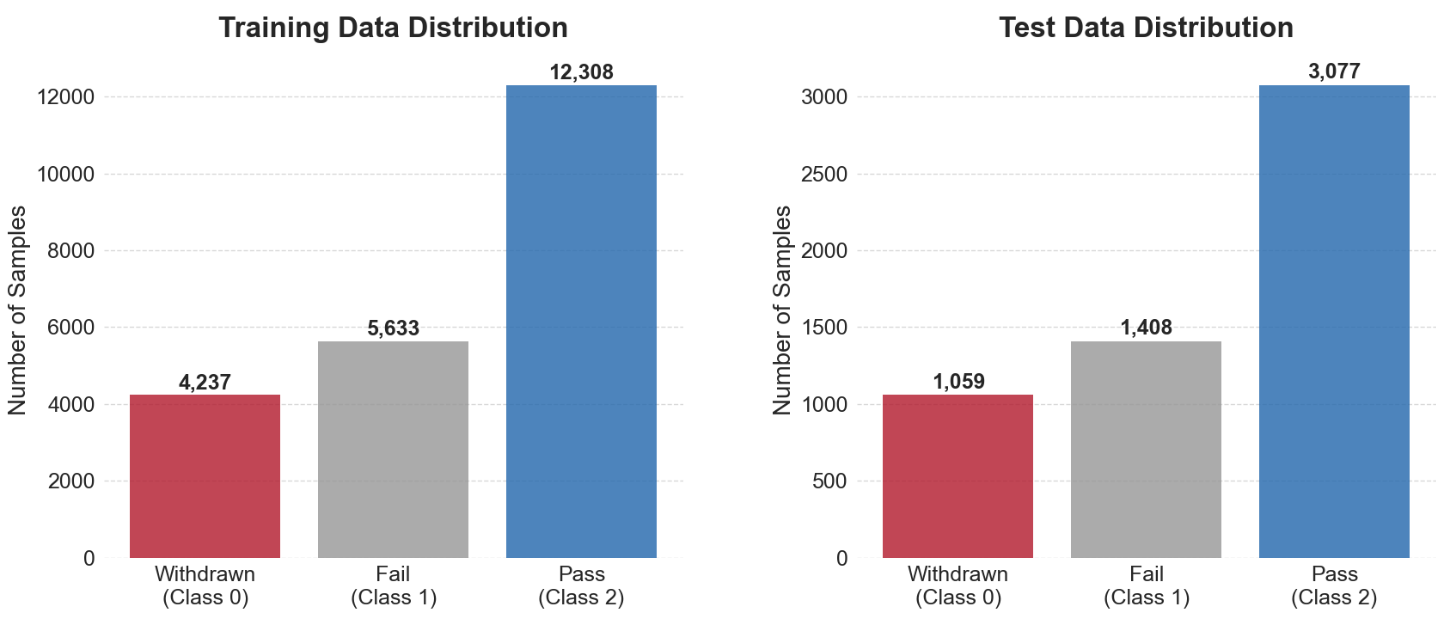
\includegraphics[width=0.9\textwidth]{../Visualizations/Report/4_1_data_class_distribution.png}
	\caption{Data Class Distribution for Training and Test Data}
	\label{fig:data_distribution}
\end{figure}

\section{Custom Weighted Analysis}
There was a notable class imbalance and a strong bias in favour of successful students in the original training dataset. With $55.5\%$ of the total samples, or $12,308$ students in the training set and $3,077$ in the test set, the {\em Pass} class (Class 2) dominated, as seen in Figure~\ref{fig:data_distribution}. With $5,633$ training samples and $1,408$ test samples, the {\em Fail} class (Class 1) made up $25.4\%$ of the dataset. With $4,237$ training samples and $1,059$ test samples, the {\em Withdrawn} class (Class 0) represented only $19.1\%$ of students, which is crucial for dropout prediction.

This distribution is further demonstrated in Figure~\ref{fig:weighted_data_class}, where the weighted distribution shows the optimisation strategy for dropout detection, and the pie chart emphasises the inherent imbalance. {\em Withdrawn} students (Class 0) received the highest weight of $2.09$ according to the weighting method outlined in Section~\ref{sec:class-weighting}. Due to their at-risk status, {\em Fail} students (Class 1) were assigned a moderate weight of $1.31$. With the lowest weight of $0.48$, {\em Pass} students (Class 2) had less of an impact on model choices. Adjusted emphasis proportions of $53.9\%$, $33.8\%$, and $12.4\%$ were the outcomes of these weights.

\begin{figure}[h]
	\centering
	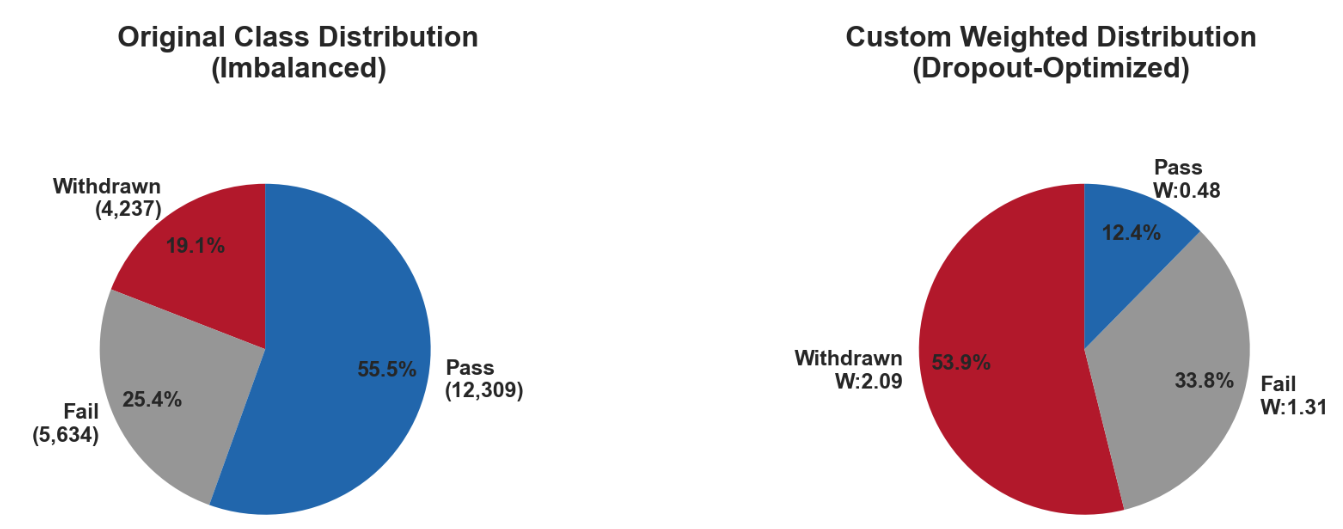
\includegraphics[width=0.9\textwidth]{../Visualizations/Report/4_2_weighted_data_class.png}
	\caption{Original vs. Weighted Class Distribution}
	\label{fig:weighted_data_class}
\end{figure}

\section{Model Performance Comparison and Rankings}
\subsection{Primary Metric Analysis: Dropout Recall Performance}
Significant differences in dropout recall performance were found when six machine learning models were evaluated, creating distinct performance hierarchies for identifying student risk. When compared to the main optimisation metric of dropout recall, the models showed different performance tiers, according to 5-fold cross-validation analysis.

With a dropout recall score of $66.8\%$, LR was the best performer and had the strongest ability to identify dropout students, according to Figure~\ref{fig:model_perfomance_comparison}. With this performance, the model showed strong predictive potential for early intervention systems, placing it well above the median threshold. SVM established a competitive alternative with comparable detection capacity, coming in second with $63.1\%$ dropout recall. Three performance levels were identified by the analysis: (i) excellent ($\geq60\%$ dropout recall), attained by LR ($66.8\%$) and SVM ($63.1\%$); (ii) good ($40$–$59\%$), represented by RF ($59.0\%$) and LightGBM ($56.0\%$); and (iii) needing improvement ($<40\%$), with KNN ($31.3\%$) and NN ($18.7\%$), both of which did not support weight customisation during training. The significant performance differences between models—a $3.7$-point difference between the top two and a $48.1$-point difference between the best and worst performers—highlight the vital significance of selecting models carefully in student support systems.

\begin{figure}[h]
	\centering
	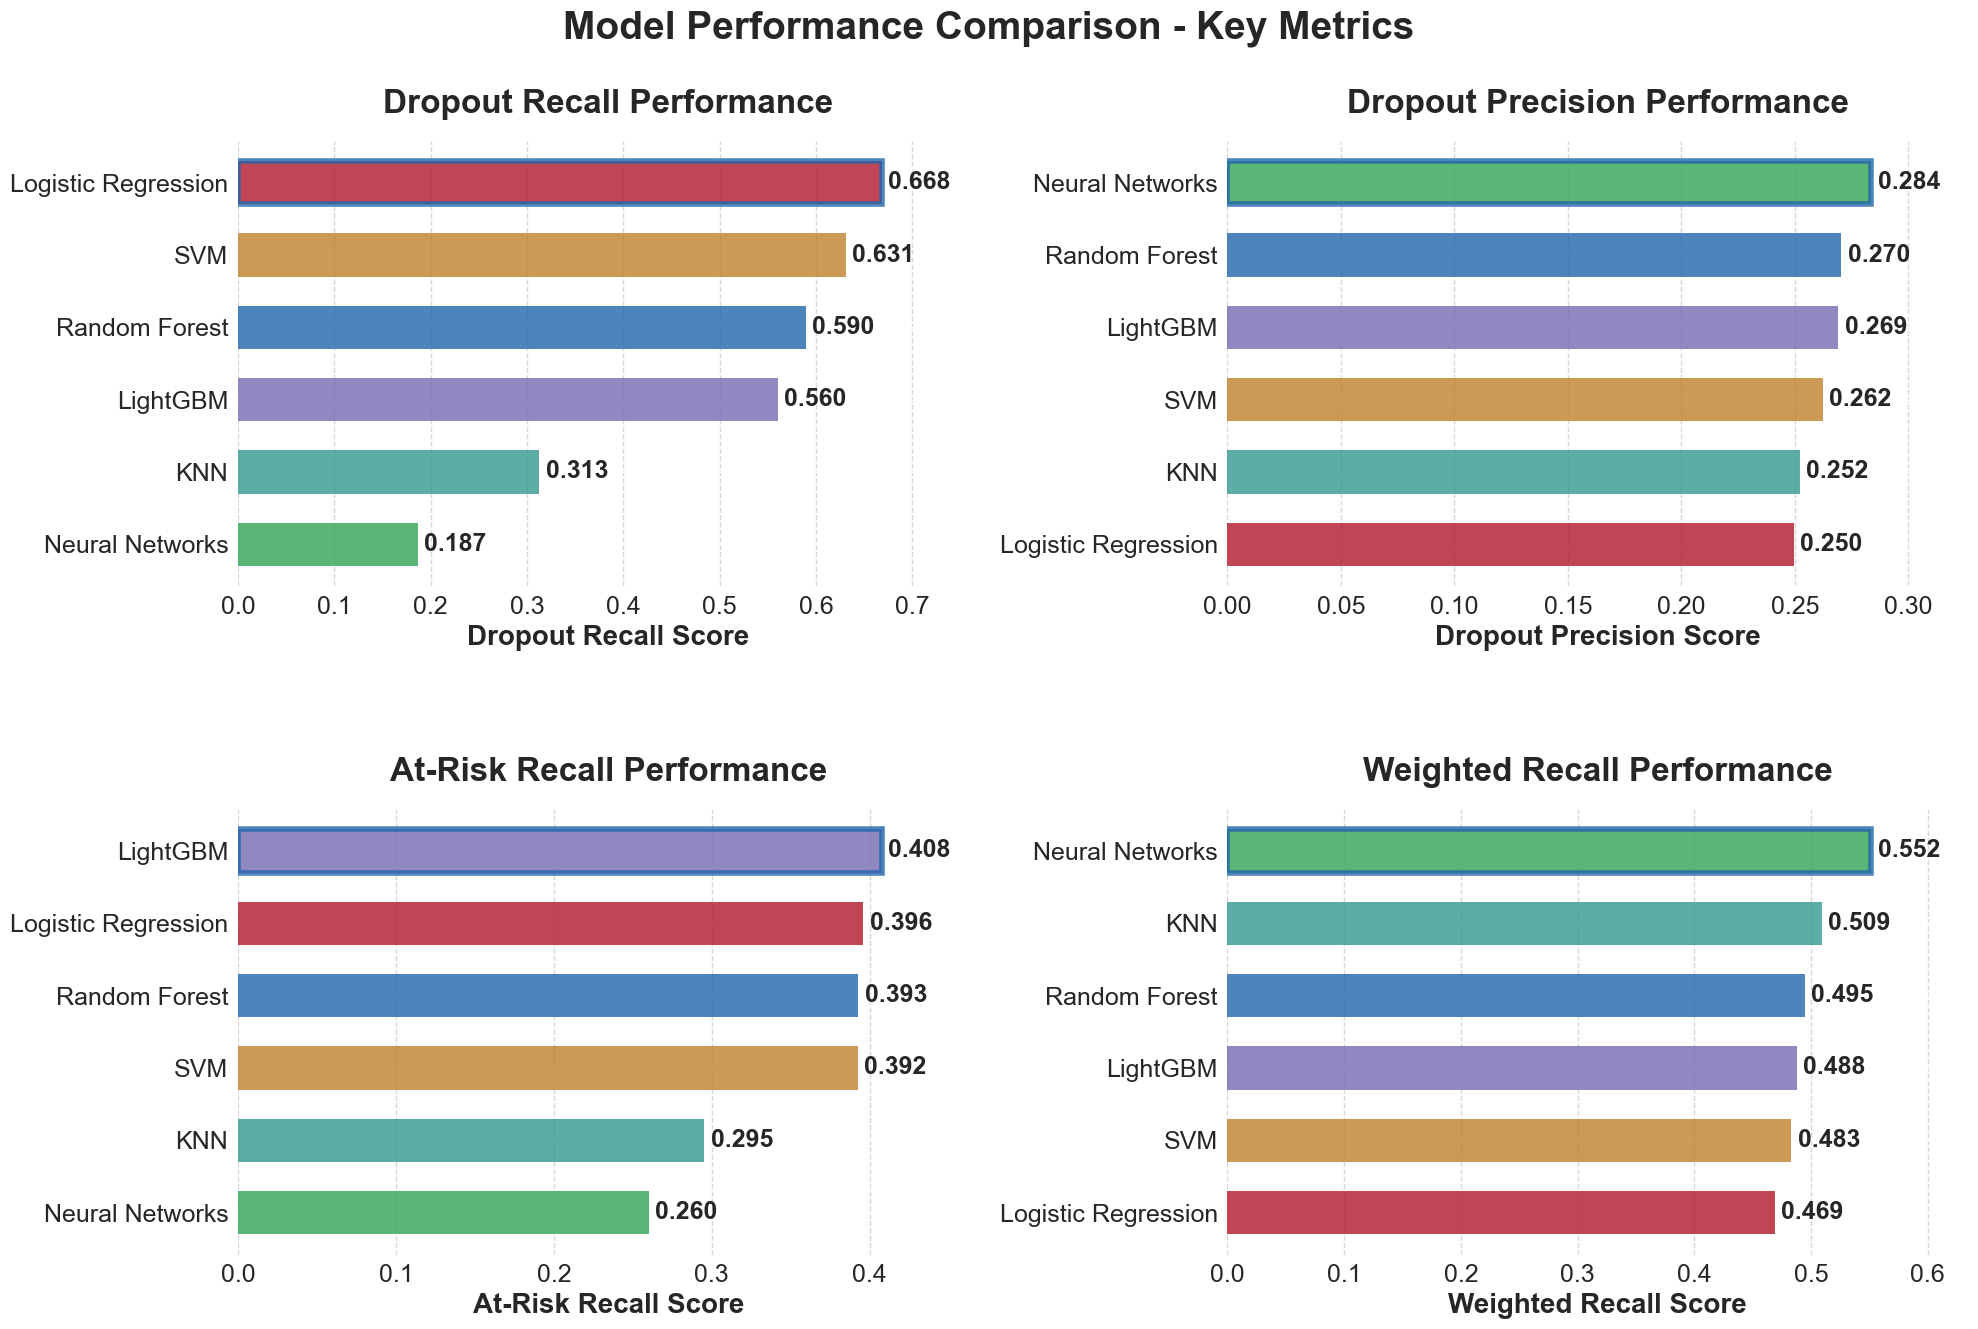
\includegraphics[width=1.0\textwidth]{../Visualizations/Report/4_3_model_performance_comparison.png}
	\caption{Model Performance Comparison}
	\label{fig:model_perfomance_comparison}
\end{figure}

\subsection{Other Multi-Metrics Performance Evaluation}
Proceeding with the examination of Figure~\ref{fig:model_perfomance_comparison}, the assessment along several performance dimensions uncovered intricate trade-offs between classification accuracy and detection capability. Although dropout recall was the main optimisation goal, dropout precision, at-risk recall, and weighted F1 scores were also taken into account in order to provide a thorough evaluation of the overall efficacy of the model.

Although recall performance was poor, NN showed superior dropout precision ($28.4\%$), indicating limited coverage of dropout students but high confidence in positive predictions. While LR recorded $25.0\%$ precision, which represents the trade-off for maximised recall performance, RF ($27.0\%$), LightGBM ($26.9\%$), and SVM ($26.2\%$) attained comparable precision levels.

In contrast to dropout recall, at-risk recall (which merges the {\em Withdrawn} and {\em Fail} classes into one) exhibited distinct rankings. The highest at-risk recall ($40.8\%$) was attained by LightGBM, which was closely followed by SVM ($39.2\%$), RF ($39.3\%$), and LR ($39.6\%$). This metric demonstrated the models' ability to detect students who need more academic assistance than just the immediate risk of dropping out.

Overall classification balance across all outcome categories was revealed by weighted F1 scores. The highest weighted F1 score ($53.0\%$) was attained by NN, which was followed by KNN ($50.7\%$) and LightGBM ($50.5\%$). These findings showed that dropout recall-optimized models inevitably compromised overall classification balance, which is consistent with the intentional design decision to give dropout student identification priority.

No single model dominated across all performance dimensions, according to the multi-metric analysis. While models with strong overall classification performance showed limited dropout detection capabilities, the top-performing models for dropout recall (LR and SVM) performed moderately in other metrics.

\section{Training Efficiency Analysis}
Significant differences in the amount of time needed for training across machine learning algorithms were found by the computational efficiency analysis. Training durations varied from 4 minutes for LR to $7.14$ hours for LightGBM, a difference of roughly $107$ times in computational demands, as shown in Figure~\ref{fig:model_training_time}. LR achieved the highest dropout recall performance ($66.8\%$) and showed remarkable efficiency with a $4$-minute training duration. Because of this combination, the algorithm was positioned as the best option for quick development cycles and real-time model updates.

NN had the lowest dropout recall performance ($18.7\%$) and required $50$ minutes of training time. Out of all the algorithms that were evaluated, this efficiency-performance combination had the least favourable profile. SVM established a reasonable efficiency-performance balance for secondary deployment consideration, achieving competitive performance ($63.1\%$ dropout recall) with $1.34$ hours of training time. Different computational requirements were shown by the intermediate performers. LightGBM required the longest training time of $7.14$ hours for $56.0\%$ performance, while RF used $3.13$ hours with $59.0\%$ dropout recall. The fact that KNN only achieved $31.3\%$ dropout recall after $1.60$ hours of training shows that there is no relationship between training time and performance results.

\begin{figure}[h]
	\centering
	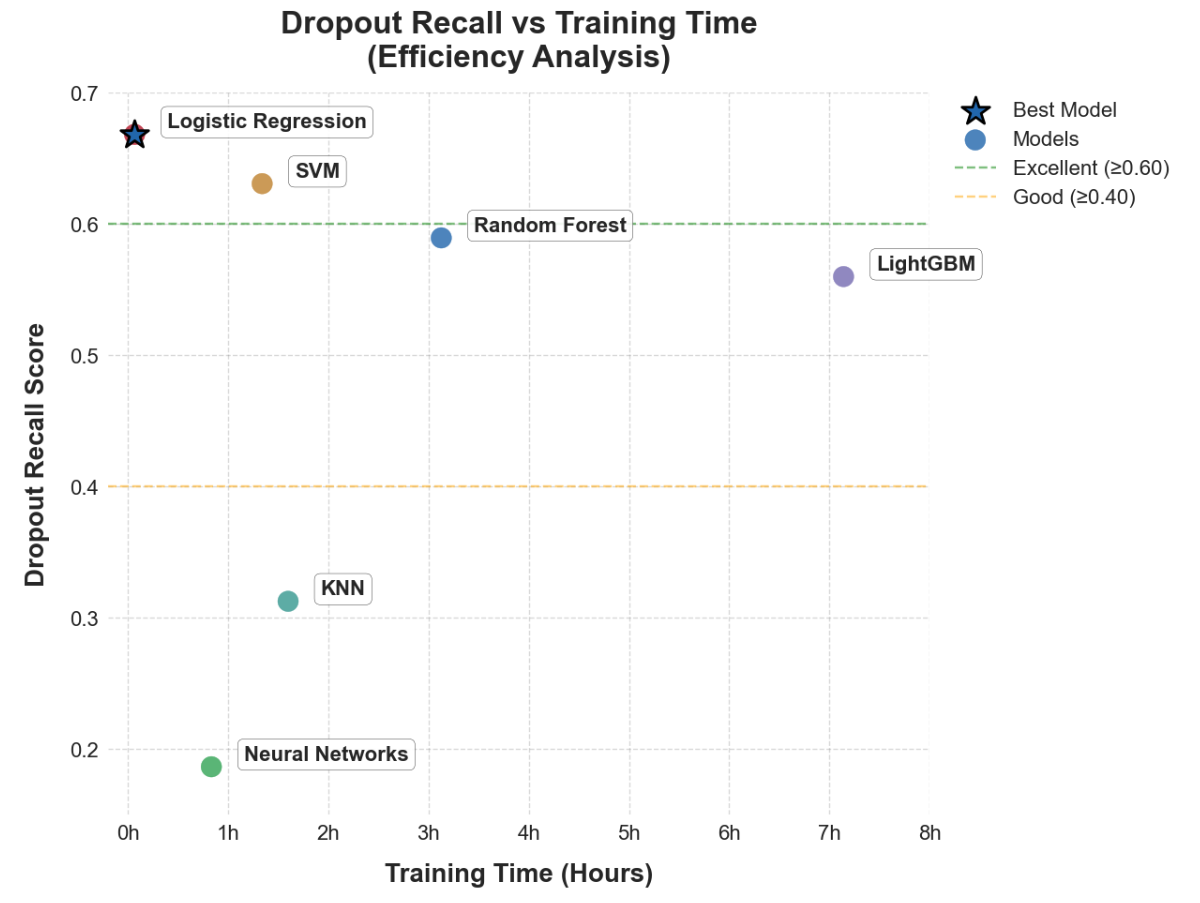
\includegraphics[width=0.9\textwidth]{../Visualizations/Report/4_4_model_training_time.png}
	\caption{Dropout Recall vs. Training Time for Six ML Models}
	\label{fig:model_training_time}
\end{figure}

\section{Hyperparameter Optimization Analysis}
Different hyperparameter space dimensionalities and optimisation requirements were reflected in the wide variations in grid search complexity among algorithms. In order to evaluate the computational overhead related to model optimisation, the analysis looked at the number of parameter combinations tested during 5-fold cross-validation.

LightGBM demonstrated the highest optimisation complexity, requiring $3,888$ parameter combinations during grid search and resulting in the longest training duration of $7.14$ hours, as illustrated in Figure~\ref{fig:model_runtime_gridSearchCV}. With $6,120$ combinations over $3.13$ hours, RF came in second, demonstrating improved parameter evaluation efficiency in spite of a larger search space. Given the small but well-explored hyperparameter space, LR's practical advantage for quick deployment is highlighted by its optimal efficiency, testing only $450$ parameter combinations in $4$ minutes. Although the additional computational investment did not result in performance gains, NN evaluated $120$ combinations in $50$ minutes, indicating moderate optimisation complexity. Lastly, SVM demonstrated targeted hyperparameter optimisation that produced efficient performance results by testing $24$ combinations in $1.34$ hours.

An inverse relationship between search complexity and performance efficiency was found by the optimisation intensity analysis. LightGBM and RF, two algorithms that required a great deal of hyperparameter exploration, used disproportionate amounts of computational resources without offering any performance benefits over more straightforward methods.

\begin{figure}[h]
	\centering
	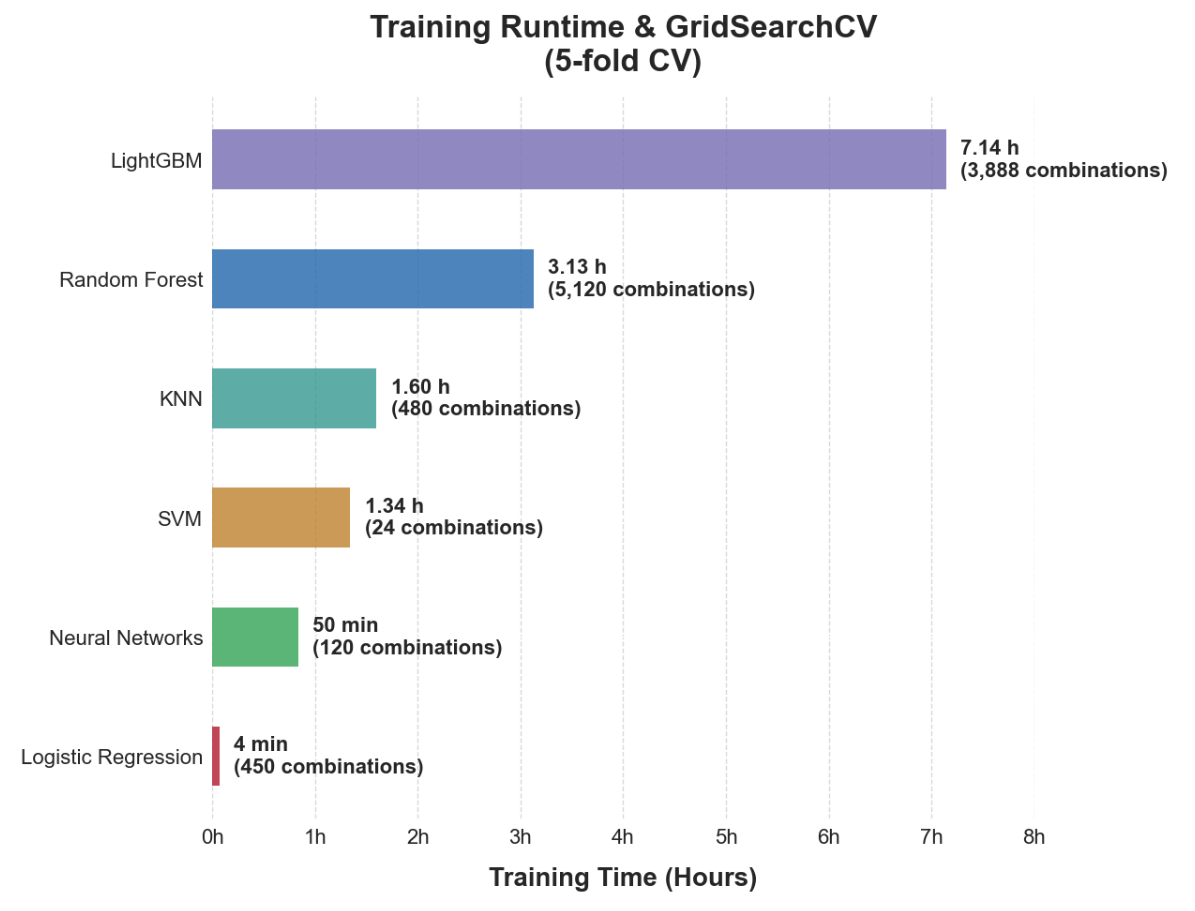
\includegraphics[width=0.9\textwidth]{../Visualizations/Report/4_5_model_runtime_gridSearchCV.png}
	\caption{Training Runtime and Parameter Combinations Across Models}
	\label{fig:model_runtime_gridSearchCV}
\end{figure}

\section{Multi-Dimensional Performance}
A five-dimensional radar plot analysis is presented in Figure~\ref{fig:radar_plot}, which offers a comprehensive visual depiction of model performance across all evaluation metrics at the same time. An alternate viewpoint for comparing the metrics of various ML models is provided by this radar plot. Performance patterns that are not apparent in single-metric comparisons are revealed by the multi-dimensional approach. To generate thorough performance profiles, the radar visualisation combines dropout recall, dropout precision, at-risk recall, weighted recall, and weighted F1 scores.

As previously found, this radar plot visualisation also shows different performance patterns among models. LR is the top performer with the largest radar area, showing balanced strength across several dimensions, including maximum dropout recall ($0.668$) and consistent performance across recall-focused dimensions. To illustrate why high weighted F1 scores do not ensure minority class identification effectiveness, NN, on the other hand, displays a highly unbalanced radar profile that is concentrated in precision and weighted F1 regions while displaying significant weaknesses in recall dimensions. Performance gradient zones highlight threshold boundaries between excellent ($\geq0.60$), good ($0.40$-$0.59$), and needs improvement ($<0.40$) levels. This allows for quick assessment of model positioning relative to deployment criteria across all evaluation dimensions at once. The radar plot's colour-coded styling distinguishes performance tiers, with excellent performers (LR, SVM) in solid bold styling, good performers (RF, LightGBM) in medium styling, and models needing improvement (KNN, NN) in lighter dashed styling.

\begin{figure}[h]
	\centering
	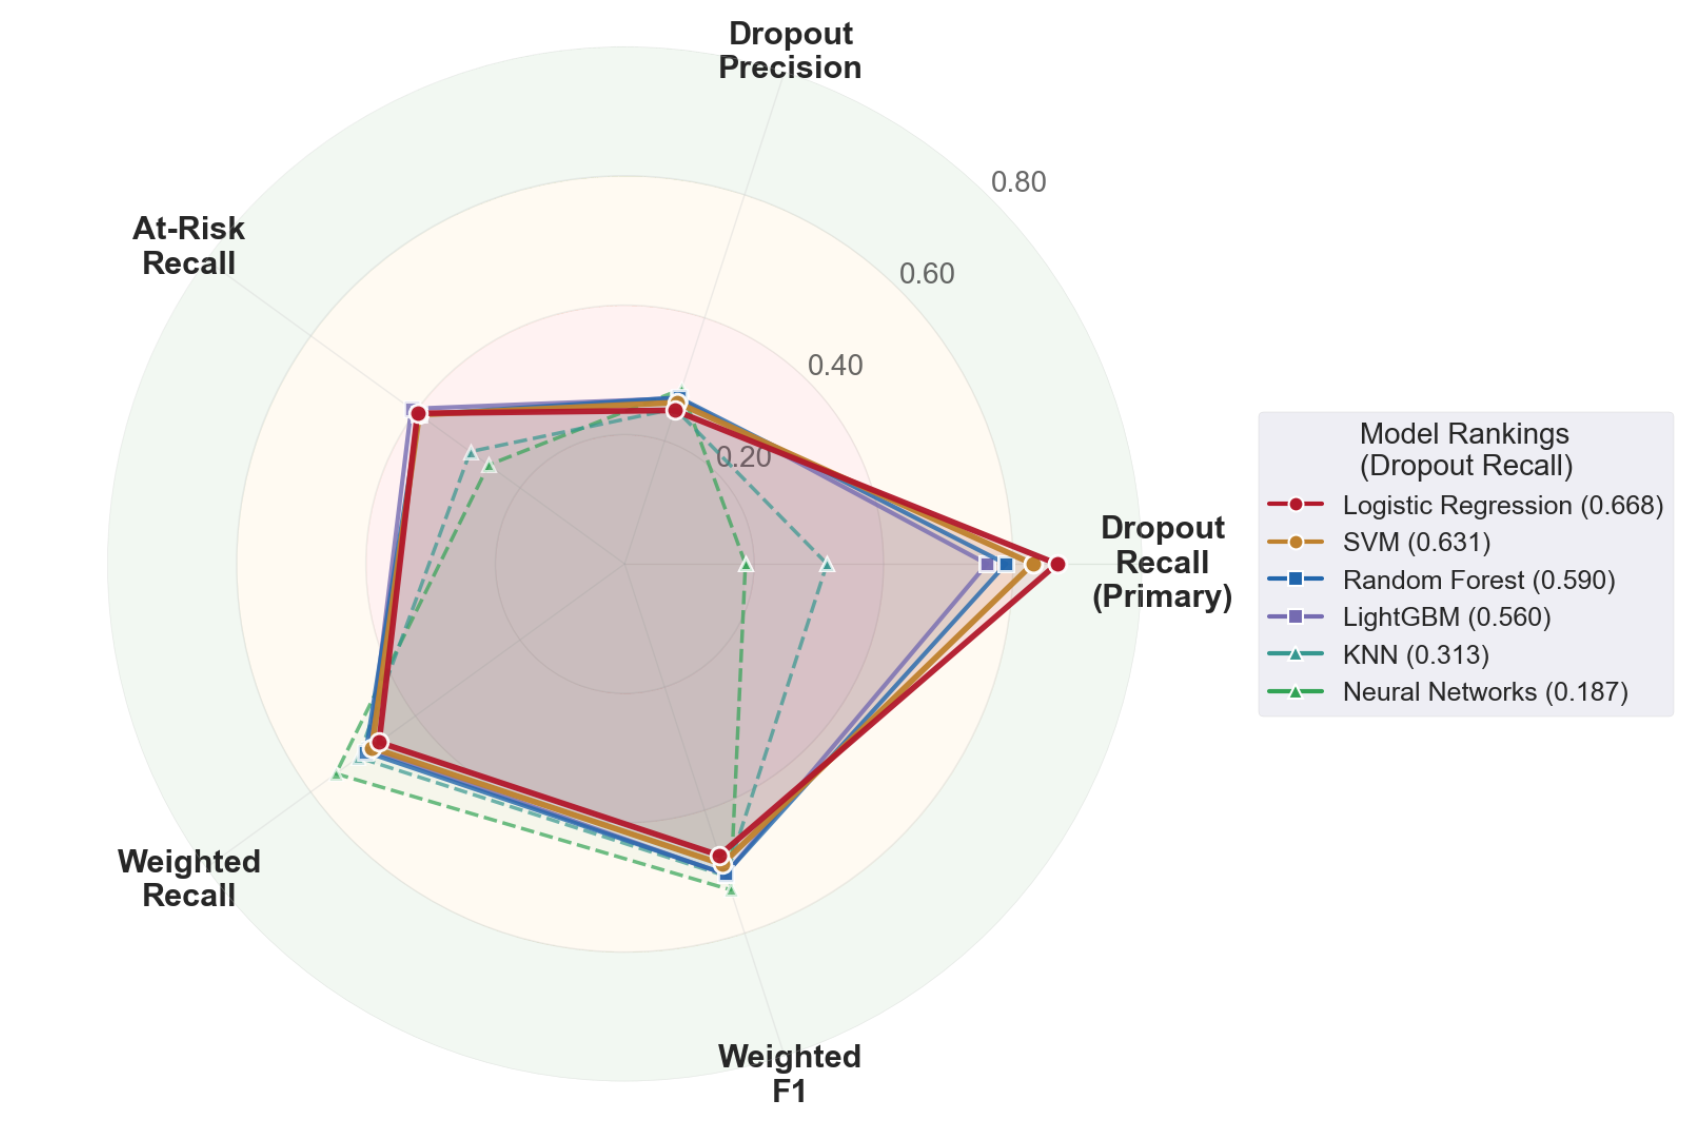
\includegraphics[width=0.9\textwidth]{../Visualizations/Report/4_6_radar_plot_comparison.png}
	\caption{Multi-metric Radar Plot for Six ML Models}
	\label{fig:radar_plot}
\end{figure}

A brief summary of the performance metrics for all assessed models is provided in Table~\ref{tab:model_performance_summary}, which combines the in-depth discussion of each machine learning model with the visual analyses that go along with it. Key metrics (at-risk recall, weighted recall, weighted F1 score, dropout recall and precision) and the associated training runtime are highlighted in the table. The dropout recall metric determines the tier classification, as previously established: models with scores above $60\%$ are classified as Top tier, those between $40$ and $60\%$ as Mid tier, and those below $40\%$ as Low tier. All things considered, the models can be clearly compared thanks to this summary table, which combines computational effectiveness and predictive performance into a single, understandable picture.

\begin{table}[h]
	\centering
	\begin{tabular}{|c|l|c|c|c|c|c|c|c|}
		\hline
		\textbf{Rank} & \textbf{Model} & 
		\makecell{\textbf{Dropout} \\ \textbf{Recall}} & 
		\makecell{\textbf{Dropout} \\ \textbf{Precision}} & 
		\makecell{\textbf{At-Risk} \\ \textbf{Recall}} & 
		\makecell{\textbf{Weighted} \\ \textbf{Recall}} & 
		\makecell{\textbf{Weighted} \\ \textbf{F1}} & 
		\makecell{\textbf{Training} \\ \textbf{Runtime}} & 
		\textbf{Tier} \\
		\hline
		\#1 & LR  & 0.668 & 0.250 & 0.396 & 0.469 & 0.474 & 4m   & Top \\
		\hline
		\#2 & SVM & 0.631 & 0.262 & 0.392 & 0.483 & 0.488 & 1.3h & Top \\
		\hline
		\#3 & RF  & 0.590 & 0.270 & 0.393 & 0.495 & 0.504 & 3.1h & Mid \\
		\hline
		\#4 & LightGBM 	& 0.560 & 0.269 & 0.408 & 0.488 & 0.505 & 7.1h & Mid \\
		\hline
		\#5 & KNN & 0.313 & 0.252 & 0.295 & 0.509 & 0.507 & 1.6h & Low \\
		\hline
		\#6 & NN  & 0.187 & 0.284 & 0.260 & 0.552 & 0.530 & 50m  & Low \\
		\hline
	\end{tabular}
	\caption{Model Performance Summary Table}
	\label{tab:model_performance_summary}
\end{table}


\section{Best Model - Multinomial Logistic Regression}
With a runtime efficiency of $4.1$ minutes, the multinomial LR emerged as the victorious machine learning model. Additional information on feature importance, performance metrics, and hyperparameter optimisation is given in this subsection.

\subsection{Hyperparameter Optimisations}
The model predicts three student outcome classes: {\em Withdrawn} (Class $0$), {\em Fail} (Class $1$), and {\em Pass} (Class $2$) using $scikit-learn$'s {\em LogisticRegression} class with the {\em SAGA} solver and $L1$ regularisation. A thorough GridSearchCV investigated $450$ parameter combinations using $5-fold$ cross-validation. Strong regularisation ($C=0.01$) and custom class weights ${0: 2.09, 1: 1.31, 2: 0.48}$, which prioritised dropout detection, were features of the ideal setup. The {\em SAGA} solver worked best for multinomial classification, and the $L1$ penalty allowed for automatic feature selection while reducing overfitting. To guarantee convergence stability, the maximum number of iterations was set at $1000$. Prioritising dropout recall over overall accuracy, the optimisation achieved $66.84\% \pm 3.08\%$ with consistent cross-fold performance, which is in line with early intervention educational goals. Although the top three configurations received identical scores, the chosen model needed the fewest maximum iterations, according to detailed hyperparameter results (Table~\ref{tab:logreg_hyperparam}). This ensures computational efficiency, which is a critical advantage for larger datasets and real-world deployment for the SDP.

\begin{table}[h]
	\centering
	\begin{tabular}{|c|c|c|c|c|c|c|}
		\hline
		\textbf{Rank} & \textbf{Score (± std)} & \textbf{C} & \textbf{l1\_ratio} & \textbf{max\_iter} & \textbf{Penalty} & \textbf{Solver} \\
		\hline
		1 & 0.6684 ± 0.0308 & 0.01 & 0.5 & 1000 & l1         & saga \\
		\hline
		2 & 0.6684 ± 0.0308 & 0.01 & 0.5 & 2000 & l1         & saga \\
		\hline
		3 & 0.6684 ± 0.0308 & 0.01 & 0.5 & 3000 & l1         & saga \\
		\hline
		4 & 0.6122 ± 0.0252 & 0.01 & 0.5 & 1000 & elasticnet & saga \\
		\hline
		5 & 0.6122 ± 0.0252 & 0.01 & 0.5 & 2000 & elasticnet & saga \\
		\hline
	\end{tabular}
	\caption{Hyperparameter exploration results for Multinomial LR using 5-fold CV}
	\label{tab:logreg_hyperparam}
\end{table}

\subsection{Confusion Matrix and Scoring Metrics Analysis}
The model was run using the multinomial LR's top-ranked hyperparameter configuration, and the resulting confusion matrix is displayed in Table~\ref{tab:confusion_matrix}. Performance patterns that are in line with the priorities of educational interventions are revealed by the analysis of this optimal multinomial LR model. The model achieved a recall rate of $65.3\%$, which closely matches the $66.84\%$ dropout recall seen during cross-validation, correctly identifying $692$ cases out of the $1,059$ actual {\em Withdrawn} students in the test set. $367$ {\em Withdrawn} students in total were incorrectly classified ($115$ predicted as {\em Fail} and $252$ as {\em Pass}), the latter being the most alarming error type because it suggests no intervention. The model's cautious prediction approach, which was influenced by conscious optimisation decisions, is reflected in this result.

The precision for Class 0 was $26.3\%$, with $692$ correct predictions out of $2,626$ ($692$ + $862$ + $1,072$) total Class 0 predictions. This indicates that for every correctly identified {\em Withdrawn} student, roughly three needless interventions were initiated. This resulted in $1,934$ false positives, including $1,072$ {\em Pass} and $862$ {\em Fail} students who were mistakenly labelled as {\em Withdrawn}. With the help of the custom class weights ${0: 2.09, 1: 1.31, 2: 0.48}$, this aggressive identification approach prioritises false positives over false negatives. This deliberate strategy aligns with educational objectives, where it is better to provide unnecessary support than to ignore {\em Fail} students. As summarised in Table~\ref{tab:scoring_metrics_report}, with an overall weighted recall of $48.08\%$ and a macro recall of $46.0\%$, the precision–recall trade-off that results shows how effective the optimisation strategy was. The effectiveness of this unbalanced optimisation design for early intervention systems is confirmed by the purposefully lower precision for Class 0 when compared to Classes 1 and 2.

\begin{table}[h]
	\centering
	\begin{tabular}{|c|c|c|c|}
		\hline
		\textbf{Actual / Predicted} & \textbf{0 - Withdrawn} & \textbf{1 - Fail} & \textbf{2 - Pass} \\
		\hline
		\textbf{0 - Withdrawn} & 692  & 115  & 252  \\
		\hline
		\textbf{1 - Fail}      & 862  & 224  & 324  \\
		\hline
		\textbf{2 - Pass}      & 1072 & 254  & 1750 \\
		\hline
	\end{tabular}
	\caption{Confusion Matrix for Multi-class Classification}
	\label{tab:confusion_matrix}
\end{table}

\begin{table}[h]
	\centering
	\begin{tabular}{|l|c|c|c|c|}
		\hline
		\textbf{Class} & \textbf{Precision} & \textbf{Recall} & \textbf{F1-Score} & \textbf{Support} \\
		\hline
		0 - Withdrawn & 0.26 & 0.65 & 0.38 & 1059 \\
		\hline
		1 - Fail      & 0.38 & 0.16 & 0.22 & 1410 \\
		\hline
		2 - Pass      & 0.75 & 0.57 & 0.65 & 3076 \\
		\hline
		\multicolumn{5}{|c|}{} \\ % <-- Empty row with edges
		\hline
		\textbf{Accuracy}   & \multicolumn{3}{c|}{0.48} & 5545 \\
		\hline
		\textbf{Macro Avg}  & 0.46 & 0.46 & 0.42 & 5545 \\
		\hline
		\textbf{Weighted Avg} & 0.56 & 0.48 & 0.49 & 5545 \\
		\hline
	\end{tabular}
	\caption{Detailed Scoring Metrics Report for Multi-class Classification}
	\label{tab:scoring_metrics_report}
\end{table}

\subsection{Feature Importance and Model Interpretability}
$L1$ regularisation made it possible to automatically select features using coefficient magnitude analysis. The feature importance ranking that resulted validated carefully crafted variables intended to predict student outcomes and showed that the top $8$ features have strong predictive power for dropout detection and distinct patterns of educational relevance.

\paragraph{Top 8 Feature Analysis} The top three features, as illustrated in Figure~\ref{fig:feature_importance}, are specifically designed variables that exhibit remarkable predictive ability for dropout detection. By capturing academic excellence through composite scoring mechanisms and validating the strategic design approach for student assessment metrics, $Excellent\_Score$ (coefficient: $0.3293$) emerged as the dominant predictor. {\em Active\_in\_VLE} (coefficient: $0.2363$) came in second with $72\%$ of the top feature's strength, effectively capturing engagement patterns in virtual learning environments that are essential for the success of online education. The engineered variable trilogy was completed by $Student\_engagement$ (coefficient: $0.1390$) at $42\%$ relative strength. It measures comprehensive student participation across multiple dimensions to provide crucial behavioural insights that complement academic performance metrics. Existing demographic and educational variables with significantly lower predictive power made up the remaining five features:  Prior educational attainment was captured by $highest\_education\_ord$ ($0.0898$, $27\%$ relative strength). Accessibility concerns were identified by $disability\_binary$ ($0.0790$, $24\%$), socioeconomic factors were represented by $imd\_band\_ord$ ($0.0234$, $7\%$), and the contributions of $age\_band\_ord$ ($0.0035$) and $region\_Wales$ ($0.0004$) were minimal. The significant decrease in coefficients from the lowest engineered variable to the highest demographic variable ($0.1390$ to $0.0898$) reinforces the strategic focus on engineered variables for educational outcome prediction and demonstrates the superior predictive value of purpose-built features over conventional student characteristics.

The multinomial LR provided good interpretability and respectable performance in the larger model comparison framework. The model is appropriate for educational stakeholders who need transparent prediction mechanisms because the linear decision boundaries made it easy to understand feature relationships.

\begin{figure}[h]
	\centering
	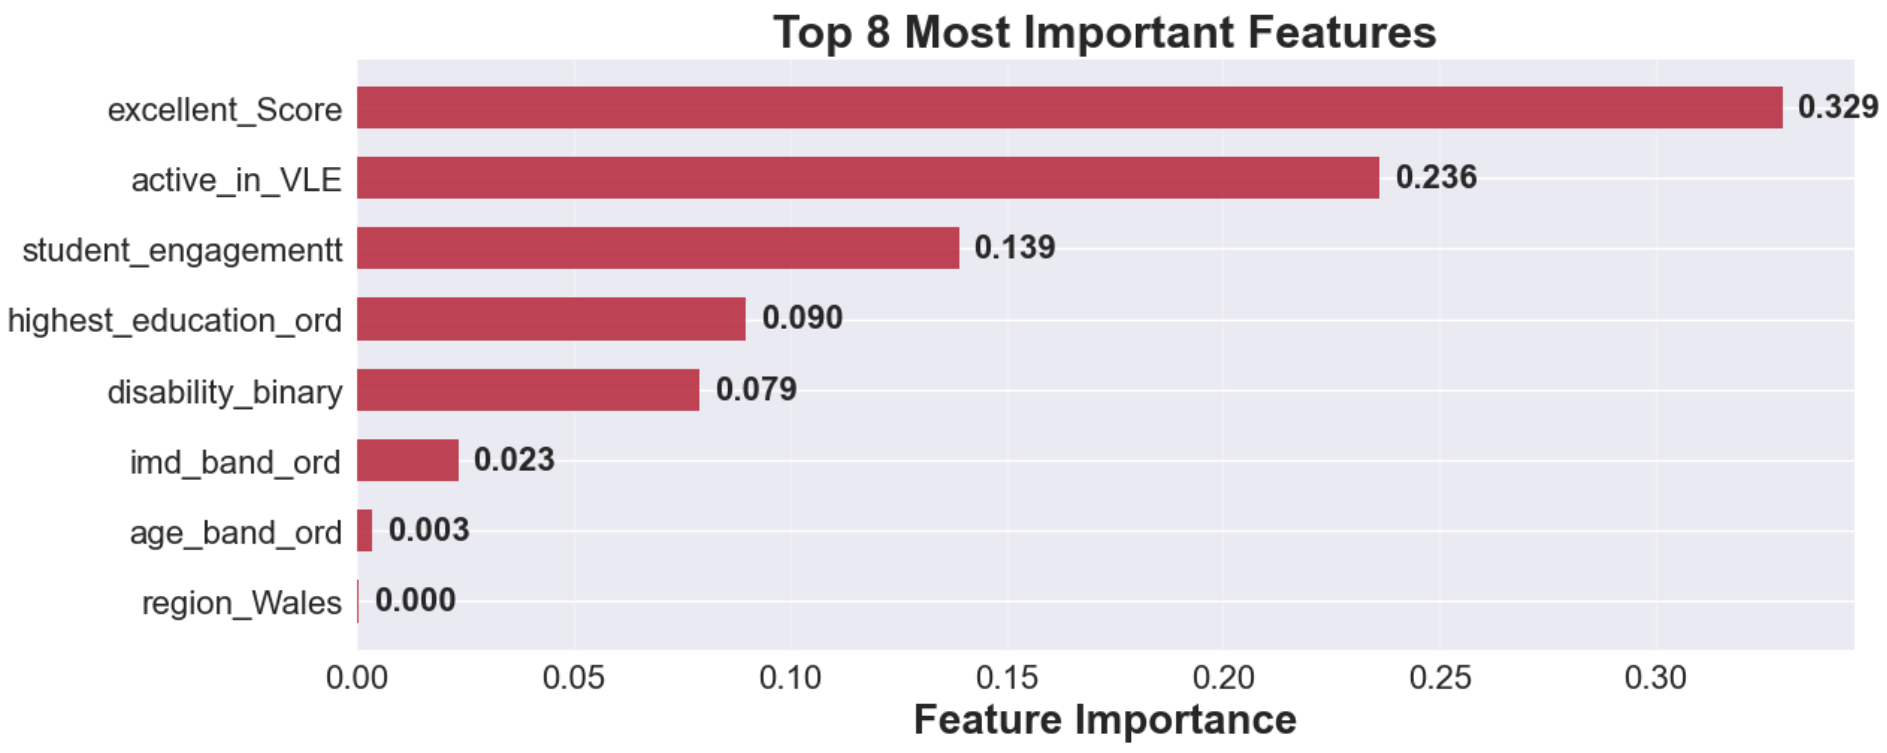
\includegraphics[width=1.0\textwidth]{../Visualizations/Report/4_7_feature_importance.png}
	\caption{Top 8 Most Important Features}
	\label{fig:feature_importance}
\end{figure}


% -----------------------------------------------------------------------------

\chapter{Further Work}
\label{chap:further_work}

\vspace{1cm}
\noindent
The following suggestions provide important avenues for expanding the six-ML model comparison framework in order to improve the robustness and performance of dropout detection.

\paragraph{Enhanced Model Optimisation and Comparison.} A methodical, cost-sensitive class-weight search should be used by all models in the current six-ML comparison. In this study, balanced weights (balanced: ${0: 1.7449, 1: 1.3123, 2: 0.6006}$; custom: ${0: 2.0939, 1: 1.3123, 2: 0.4805}$) were compared to a single custom weighting scheme. Future research should expand on this strategy by looking for multipliers across a grid for each of the six models. This would directly maximise the $dropout-recall$ objective while maintaining stability across folds and cohorts (for example, multipliers of +$20$/$0$/$-20\%$). A structured workshop with academic advisors, educational stakeholders, and domain experts could help pre-narrow the weight space by incorporating domain priors on false-negative costs. These expert-informed choices would then be confirmed by an empirical search across the whole model suite. The Class Weighting Strategy presented in Table~\ref{tab:class_weight} and Section~\ref{sec:class-weighting} is expanded upon in this procedure. Instead of depending only on ad hoc re-weighting, the six-ML comparison should also assess sampling strategies and principled loss functions in addition to weighting schemes. Modern strategies like Class-Balanced losses, as described in the background (in Section~\ref{sec:strategies_imbalanced_data}), provide theoretically sound substitutes; evaluating these in addition to focal loss across all six models would demonstrate whether principled objectives routinely perform better than fixed multipliers. Finally, adopting class-aware resampling or implementing weighted cross-entropy within NN frameworks would restore equitable comparison conditions for models (KNN, NN) that lack native class-weighting mechanisms (in Table~\ref{tab:class_weight}).

\paragraph{Temporal Modelling and Validation.} In order to detect dropout risk earlier, the six-ML comparison framework should be expanded to include temporal and survival-style modelling. In order to identify which algorithms best capture behavioural changes over successive assessments and seasonal patterns in student activity, future iterations should evaluate multi-temporal windows across all six models, even though this study limited features to the window before the first assessment (Subsection~\ref{subsec:defining_TMA}). Furthermore, the validation strategy needs to be expanded beyond the current 5-fold CV and cohort+outcome stratification split (Section~\ref{sec:data_stratification}). A more thorough method would test robustness under cohort shift by methodically evaluating all six models using temporal hold-outs and leave-one-module-presentation-out validation. In order to ensure more equitable comparisons across the algorithm suite, nested CV should also be used to lessen bias in model selection.

% -----------------------------------------------------------------------------

\chapter{Conclusion}
\label{chap:conclusion}

\vspace{1cm} 
\noindent
This study created a comparative ML pipeline to anticipate student withdrawal early and facilitate prompt intervention in a virtual learning environment (VLE), as high attrition in VLEs continues to be a persistent challenge. The problem was constructed as a three-class task with {\em Withdrawn} (Class 0), {\em Fail} (Class 1), and {\em Pass} (Class 2) using the OULAD dataset. Through a seven-phase workflow that covered data ingestion to model selection, the goals were to integrate engagement-aware features, socio-demographic signals, and find a workable model for early detection. Early behavioural indicators, such as $excellent\_score$, {\em active\_in\_VLE}, and a composite $student\_engagement$ flag, were designed around the first {\em TMA} window. Custom weights ($0: 2.09, 1: 1.31, 2: 0.48$) and a dropout-recall-oriented goal were used to address class imbalance. RF, Multinomial LR, KNN, LightGBM, SVM, and NN were the six algorithms that were compared using the same split and scoring criteria. With $19.1\%$ {\em Withdrawn}, $25.4\%$ {\em Fail}, and $55.5\%$ {\em Pass}, the dataset showed an unbalanced class distribution (Table~\ref{tab:class_distribution_merge}). The socio-demographic analysis revealed modest gender differences but distinct gradients for age, disability, IMD band, and prior education (Table~\ref{tab:var_selection}), all of which were kept for modelling and interpretation, with the exception of gender.

\vspace{0.2cm} 
According to the model comparison, Multinomial LR outperformed SVM at $63.09\%$ and achieved the highest {\em Withdrawn} recall at $66.84\%$, exceeding the study's goal of $\geq60\%$. KNN and NN performed poorly for the minority class, whereas RF and LightGBM formed a mid-tier (Table~\ref{tab:model_performance_summary}). Given its high recall of the class of greatest institutional interest, this ranking supports the choice of LR for production. While SVM took about $1.34$h, RF $3.13$h, and LightGBM $7.14$h for lower or mid-tier recall, the final LR model was trained in 5-fold CV in about $4$ minutes, allowing for quick iteration and re-training (Figure~\ref{fig:model_training_time}). For regular refreshes and operational use, LR is therefore preferred by the time-to-value profile. The LR confusion matrix revealed the intended bias towards recall in relation to the precision–recall trade-off: {\em Withdrawn} recall reached $65.3\%$ while precision was $26.3\%$ (Table~\ref{tab:scoring_metrics_report}). In actuality, more students were flagged than withdrew, which is consistent with early-warning needs where it is more expensive to check for missing {\em Withdrawn} students than to perform additional checks. This behaviour is also expected under the custom weights and objective.

\vspace{0.2cm} 
Engagement variables dominated the LR coefficients in terms of feature importance and interpretation, with $student\_engagement$ ranking third, {\em active\_in\_VLE} second, and $excellent\_score$ first (Figure~\ref{fig:feature_importance}). This demonstrated the high predictive value of straightforward and understandable engagement proxies prior to {\em TMA1}. Age and regional dummies had little effect on socio-demographics, but $highest\_education$, $disability$, and $imd\_band$ all contributed significant but smaller signals. These results give employees clear explanations, demonstrating that lower withdrawal risk is associated with better early performance and above-average activity. The following is a summary of the research objectives, which were met:

\begin{itemize}
	\item Engagement features in the models: The three engineered engagement indicators were used and proved to be the best predictors in the winning ML model.
	\item Socio-demographic associations: Highest education, IMD, and disability all demonstrated significant correlations with outcomes in the quantified and visual relationships; gender was left out because of the lack of practical separation.
	\item Selecting a useful model: The $\geq60\%$ recall target was successfully met by LR, which was chosen for its leading recall, short runtime, and interpretability.
\end{itemize}

Given the modest precision observed, advisors should triage the flagged list of students who are most likely to withdraw after the chosen LR model has been used as a first-line screener (Table~\ref{tab:scoring_metrics_report}). While thresholds and class weights can be adjusted to local capacity, this process can be supported by straightforward rules like verifying current activity, checking recent {\em TMA} outcomes, and cross-referencing support history. Since some flagged cases will still result in passing, communication with students should continue to be constructive rather than punitive. OULAD's daily click-log granularity and the UK context set boundaries for external validity in terms of scope and limitations. In order to produce clean ``pre-assessment" features, the method also depends on {\em TMA1} timing assumptions. Additionally, the investigation of alternative weighting or loss strategies and broader temporal modelling were restricted by resource limitations. These limitations influence how the findings are interpreted and how broadly they can be applied to other VLEs.

\vspace{0.4cm} 
\noindent
To conclude, this project provided a clear, socio-economically informed, engagement-aware pipeline for early withdrawal detection. The comparison proved that a regularised multinomial LR can successfully strike a balance between speed, interpretability, and performance, which makes it appropriate for promptly identifying students who are at risk. With human-in-the-loop review, institutions can use it to address the precision trade-off while addressing surface withdrawal risks. For further research, there are opportunities to improve temporal modelling, increase optimisation, and improve fairness controls. The main goal, which was to offer useful and comprehensible predictions that aid in better retention choices in online learning, was ultimately accomplished.

% =============================================================================

% Finally, after the main matter, the back matter is specified.  This is
% typically populated with just the bibliography.  LaTeX deals with these
% in one of two ways, namely
%
% - inline, which roughly means the author specifies entries using the 
%   \bibitem macro and typesets them manually, or
% - using BiBTeX, which means entries are contained in a separate file
%   (which is essentially a database) then imported; this is the 
%   approach used below, with the databased being dissertation.bib.
%
% Either way, the each entry has a key (or identifier) which can be used
% in the main matter to cite it, e.g., \cite{X}, \cite[Chapter 2}{Y}.

\backmatter

%\bibliographystyle{unsrt}
\bibliography{sample_bibtex.bib}

% -----------------------------------------------------------------------------

% The dissertation concludes with a set of (optional) appendices; these are 
% the same as chapters in a sense, but once signalled as being appendices via
% the associated macro, LaTeX manages them appropriately.

\appendix

\chapter{Socio-Demographic Visualisations}
\label{appx:socio_demographic_plots}

The linear regression analyses in this appendix look at the correlation between six important socio-demographic factors and student outcomes ({\em Pass, Fail, Withdrawn}). To comprehend how various demographic factors affect academic performance and dropout patterns, each variable is examined independently. Gender, age band, disability status, highest education level, income deprivation (IMD) band, and region are the six socio-demographic factors that were looked at. The proportionate results across the demographic categories are displayed by fitting three regression lines for each variable; the slopes and $R^2$ values show the direction and strength of each relationship.

\begin{figure}[h]
	\centering
	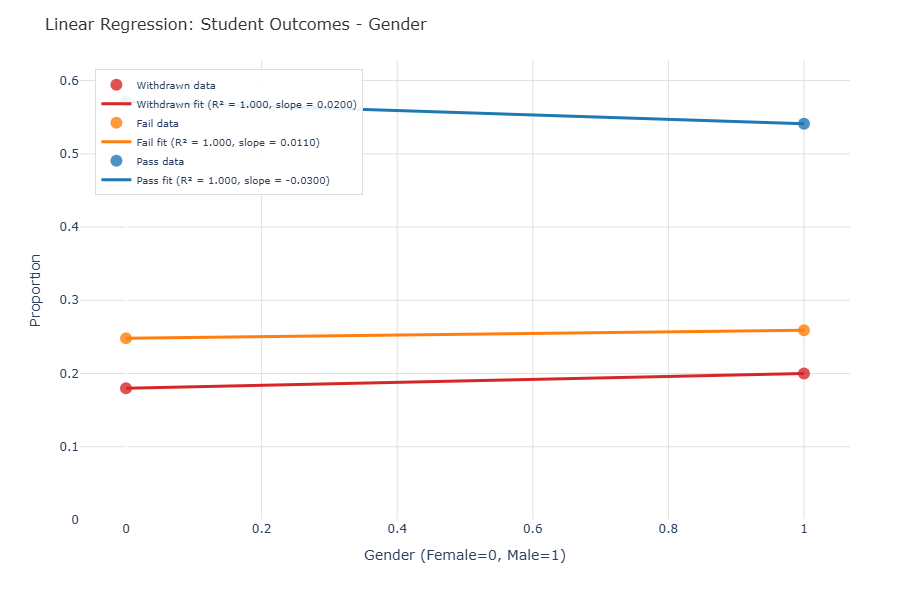
\includegraphics[width=0.9\textwidth]{../Visualizations/Report/A1_Gender_plot.png}
	\caption{Student Outcomes by Gender}
	\label{gender_plot}
\end{figure}
\begin{figure}[h]
	\centering
	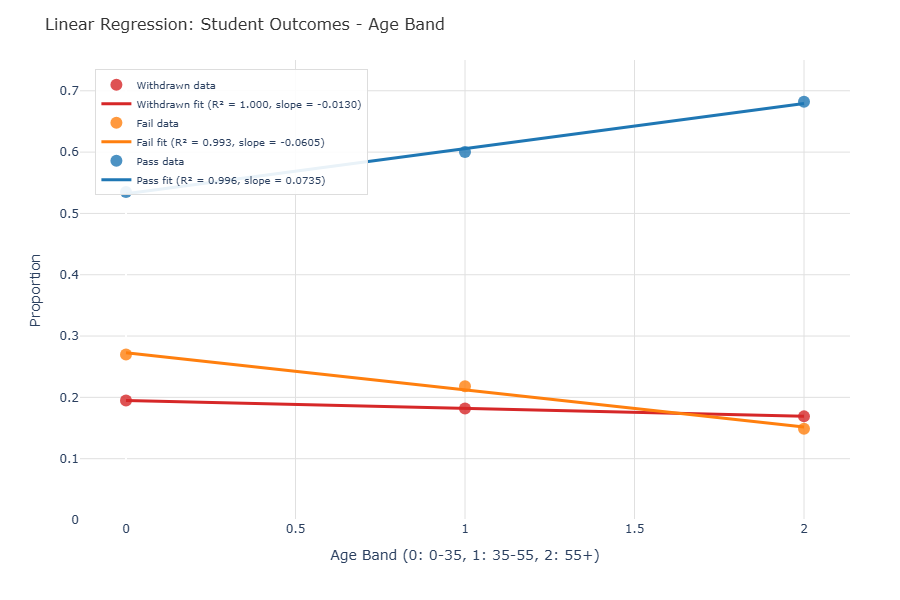
\includegraphics[width=0.9\textwidth]{../Visualizations/Report/A1_Age_band_plot.png}
	\caption{Student Outcomes by Age Band}
	\label{age_band_plot}
\end{figure}
\begin{figure}[h]
	\centering
	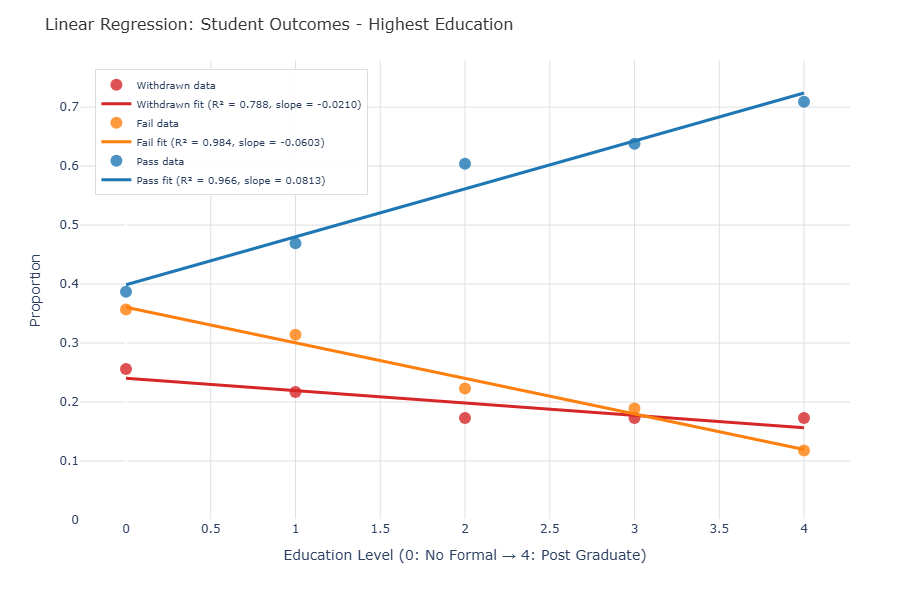
\includegraphics[width=0.9\textwidth]{../Visualizations/Report/A1_HE_plot.png}
	\caption{Student Outcomes by Highest Education Level}
	\label{HE_plot}
\end{figure}
\begin{figure}[h]
	\centering
	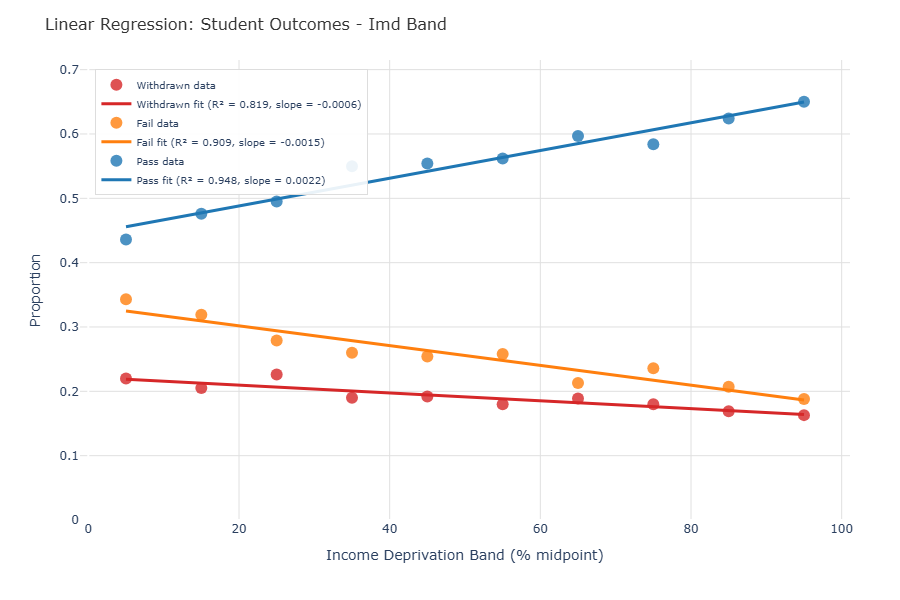
\includegraphics[width=0.9\textwidth]{../Visualizations/Report/A1_IMD_band_plot.png}
	\caption{Student Outcomes by IMD band}
	\label{IMD_plot}
\end{figure}
\begin{figure}[h]
	\centering
	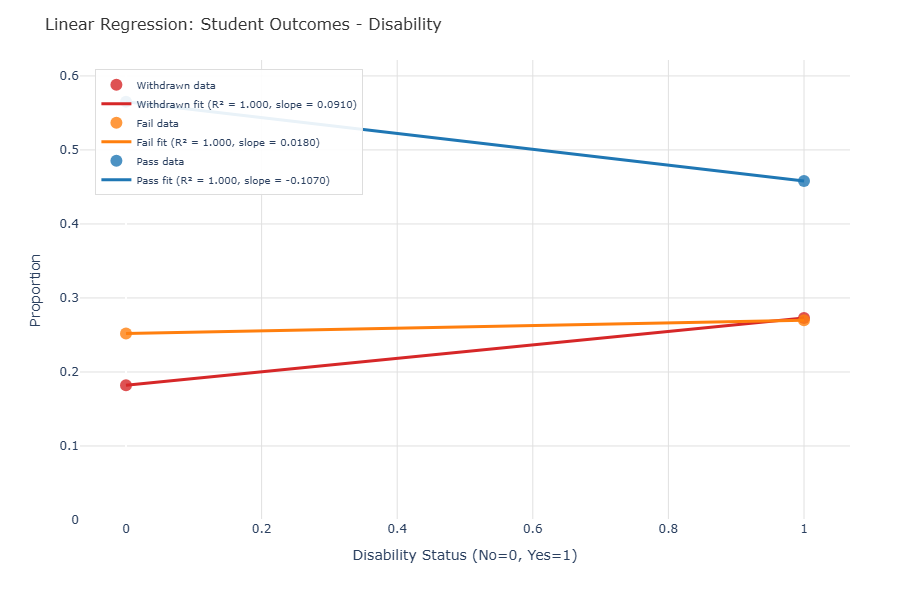
\includegraphics[width=0.9\textwidth]{../Visualizations/Report/A1_Disability_plot.png}
	\caption{Student Outcomes by Disability Level}
	\label{disability_plot}
\end{figure}
\begin{figure}[h]
	\centering
	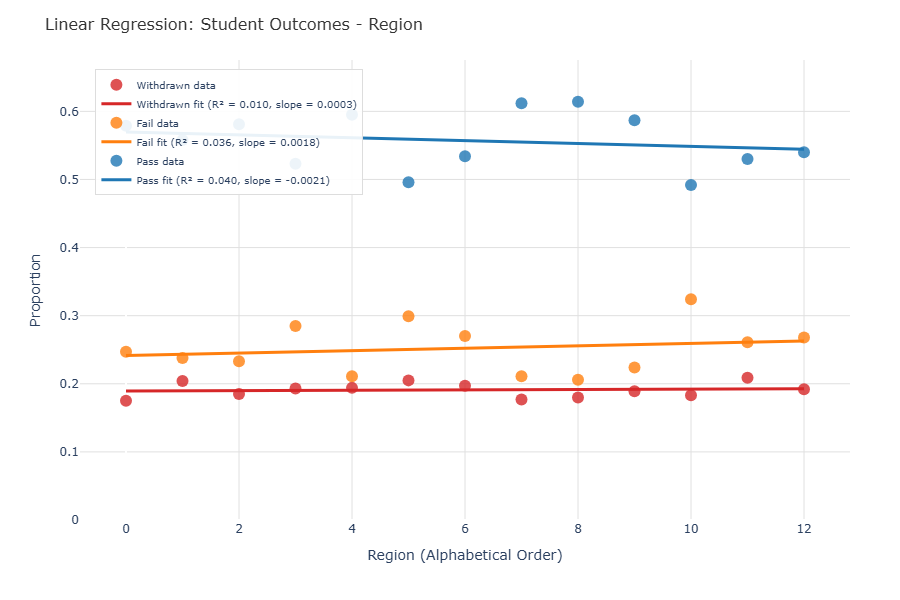
\includegraphics[width=0.9\textwidth]{../Visualizations/Report/A1_Region_plot.png}
	\caption{Student Outcomes by UK Region}
	\label{Region_plot}
\end{figure}


\noindent
%Note that in line with most research conferences, the examiners are not
%obliged to read such appendices.

% =============================================================================

\end{document}
